\documentclass[ms,cpyr,lof,lot]{uathesis}





\usepackage{graphicx}
\usepackage{amsmath,amssymb}
\usepackage{xcolor}
\usepackage{mathtools}
\usepackage{etoolbox}
\usepackage{booktabs}
\usepackage{float}
\usepackage{graphicx}
\usepackage{geometry}
\usepackage{multicol}
\usepackage{caption}
\usepackage{natbib}
\usepackage{siunitx}
\usepackage{listings}
\usepackage{bm}
\usepackage[outdir=./eps2pdf/]{epstopdf}
\graphicspath{
  {figures/}
  {figures/goals/}
  {figures/light_data/}
  {figures/attenuation/}
}


\setlength{\tabcolsep}{12pt}

\definecolor{commentcolor}{HTML}{752000}
\definecolor{keywordcolor}{HTML}{007520}

\lstset{
    language=[90]Fortran,
    inputpath=../kelp/code/fortran/src,
    basicstyle=\linespread{0.8}\ttfamily,
    commentstyle=\rmfamily,
    keywordstyle=\color{commentcolor},
    commentstyle=\color{keywordcolor},
    showstringspaces=false,
    numbers=left,
    breaklines=true,
    numbersep=1em,
    frame=leftline,
    tabsize=4,
    xleftmargin=.5in,
    xrightmargin=.5in}

\DeclareMathOperator{\atantwo}{atan2}

\newcommand\xmin{x_{\mbox{min}}}
\newcommand\xmax{x_{\mbox{max}}}
\newcommand\ymin{y_{\mbox{min}}}
\newcommand\ymax{y_{\mbox{max}}}
\newcommand\zmin{z_{\mbox{min}}}
\newcommand\zmax{z_{\mbox{max}}}

\newcommand\plotwidth{7in}


\newcommand{\ds}{\displaystyle}

\newcommand{\erf}{\mbox{erf}}
\newcommand{\sign}{\mbox{sign}}
\newcommand{\ceil}{\mbox{ceil}}
\newcommand{\floor}{\mbox{floor}}
\newcommand\R{\mathbb{R}}
\newcommand\norm[1]{||#1||}
\newcommand\LL{\mathcal{L}}
\newcommand\FF{\mathcal{F}}


\newcommand\NN{\mathbb{N}}
\newcommand\RR{\mathbb{R}}
\newcommand\CC{\mathbb{C}}
\newcommand\BB{\mathcal{B}}
\newcommand\DD{\mathcal{D}}
\newcommand\QQ{\mathcal{Q}}
\newcommand\unorm[1]{\left\lVert #1 \right\rVert_\infty}
\newcommand\ip[1]{\left\langle #1 \right\rangle}
\newcommand\abs[1]{\left| #1 \right|}
\newcommand\conj\overline
\newcommand\pd[2]{\frac{\partial #1}{\partial #2}}
\newcommand{\iter}[1]{^{(#1)}}
\newcommand\qed{\hfill$\blacksquare$\hspace{0.5in}}

\newcommand\nomega{{n_{\vec{\omega}}}}


\title{Modelling the Light Field in Macroalgae Aquaculture}
\author{Oliver Graham Evans}
\conferraldate{May}{2018}

\advisor{Dr. Kevin Kreider}
\chair{Dr. Kevin Kreider}
\collegedean{Dr. John Green}
\gradschdean{Dr. Chand Midha}
\coadvisor{Dr. Curtis Clemons}
\facreader{Dr. Gerald Young}

\begin{document}

\maketitle
\chapter{INTRODUCTION} \label{ch:intro}

\section{Motivation}
  Given the global rise in population, efficient and innovative resource utilization is increasingly important.
In particular, food and fuel are clearly in high demand.
Meanwhile, growing concern for the negative environmental impacts of petroleum-based fuel is generating a market for biofuel, especially corn-based ethanol.
However, corn-based ethanol has been heavily criticized for diverting land usage away from food production.
At the same time, a great deal of unutilized saltwater coastline is available for both food and fuel production through seaweed cultivation.
Specifically, the sugar kelp \textit{Saccharina Latissima} is known to be a viable source of food, both for direct human consumption and for fish cultivation, as well as for biofuel production.

Furthermore, nitrogen leakage into water bodies is a significant ecological danger, and is especially relevant near large conventional agriculture facilities due to run-off from nitrogen-based fertilizers, as well as near wastewater treatment plants.
As a specific example, there is a wastewater treatment plant in Boothbay Harbor, Maine which is facing increasingly demanding EPA regulations limiting the concentration of certain nutrients permissible to be released into the ocean via wastewater treatment outfalls.
In order to adhere to these stricter requirements using conventional nutrient remediation, a significant quantity of specialized equipment would be necessary, which is not currently present in the Boothbay Harbor plant.
Being surrounded on all sides by water and private property, the treatment plant lacks the necessary space for the additional equipment, and would therefore need to move their entire facility to a new location in order to conform to these new nutrient regulations.
As an alternative to conventional nutrient remediation techniques, the cultivation of the macroalgae \textit{Saccharina Latissima} (sugar kelp) near the outfall site has been proposed.
The purpose of such an undertaking would be twofold: to prevent eutrophication of the surrounding ecosystem by sequestering the nutrients in question, and to reduce the need for nutrient input, which is one of the largest costs in macroalgae cultivation. 

Once grown, a variety of products can be derived from macroalgae, including biofuel, fish/cattle feed stock, and high value chemical materials such as alginate and agar.
Food for human consumption is also a common product of kelp aquaculture, though it may not be ideal for a wastewater treatment application.
Thus, there is an ongoing effort to investigate the feasibility, and optimal implementation of kelp farming in wastewater treatment operations. 

Industrial scale macroalgae cultivation has long existed in Eastern Asia due to the popularity of seaweed in Asian cuisine.
  More recently, kelp aquaculture has been developing in Scandinavia and in the Northeastern United States.
For example, the MACROSEA project is a four year international research collaboration funded by the Research Council of Norway targeting ``successful and predictable production of high quality biomass thereby making significant steps towards industrial macroalgae cultivation in Norway.'' 
The project includes both cultivators and scientists, working to develop a precise understanding of the full life cycle of kelp and its interaction with its environment.
A fundamental aspect of this endeavor is the development of mathematical models to describe the growth of kelp.
Work is underway at SINTEF, a private Norwegian research institution, to develop such models.
Ole Jacob Broch is a mathematician at SINTEF, a research organization in Trondheim, Norway, who has been working to model the growth of \textit{Saccharina Latissima} using SINMOD, a large-scale 3D hydrodynamical ocean model developed at SINTEF which generates data on water temperature, water velocity, light intensity, and phytoplankton concentrations among other valuable quantities \cite{wassmann_modelling_2006}.

One aspect of the model which has yet to be fully developed is the availability of light, considering factors such as absorption and scattering by the aquatic medium, as well as by the kelp itself.
In this thesis, we contribute to this effort by developing a first-principles model of the light field in a kelp farming environment.
As a first step, a model for the spatial distribution of kelp is developed.
Radiative transfer theory is then applied to determine the effects of the kelp and water on the availability of light throughout the medium.
We pursue a numerical finite difference solution to the Radiative Transfer Equation, and subsequently discuss asymptotic approximations which prove to be sufficiently accurate and less computationally intensive.
We also provide a detailed description of the numerical solution of this model, accompanied by source code for a FORTRAN implementation of the solution.
This model can be used independently, or in conjunction with a life cycle kelp model to determine the amount of light available for photosynthesis at a single time step.

\begin{figure}[h]
  \centering
  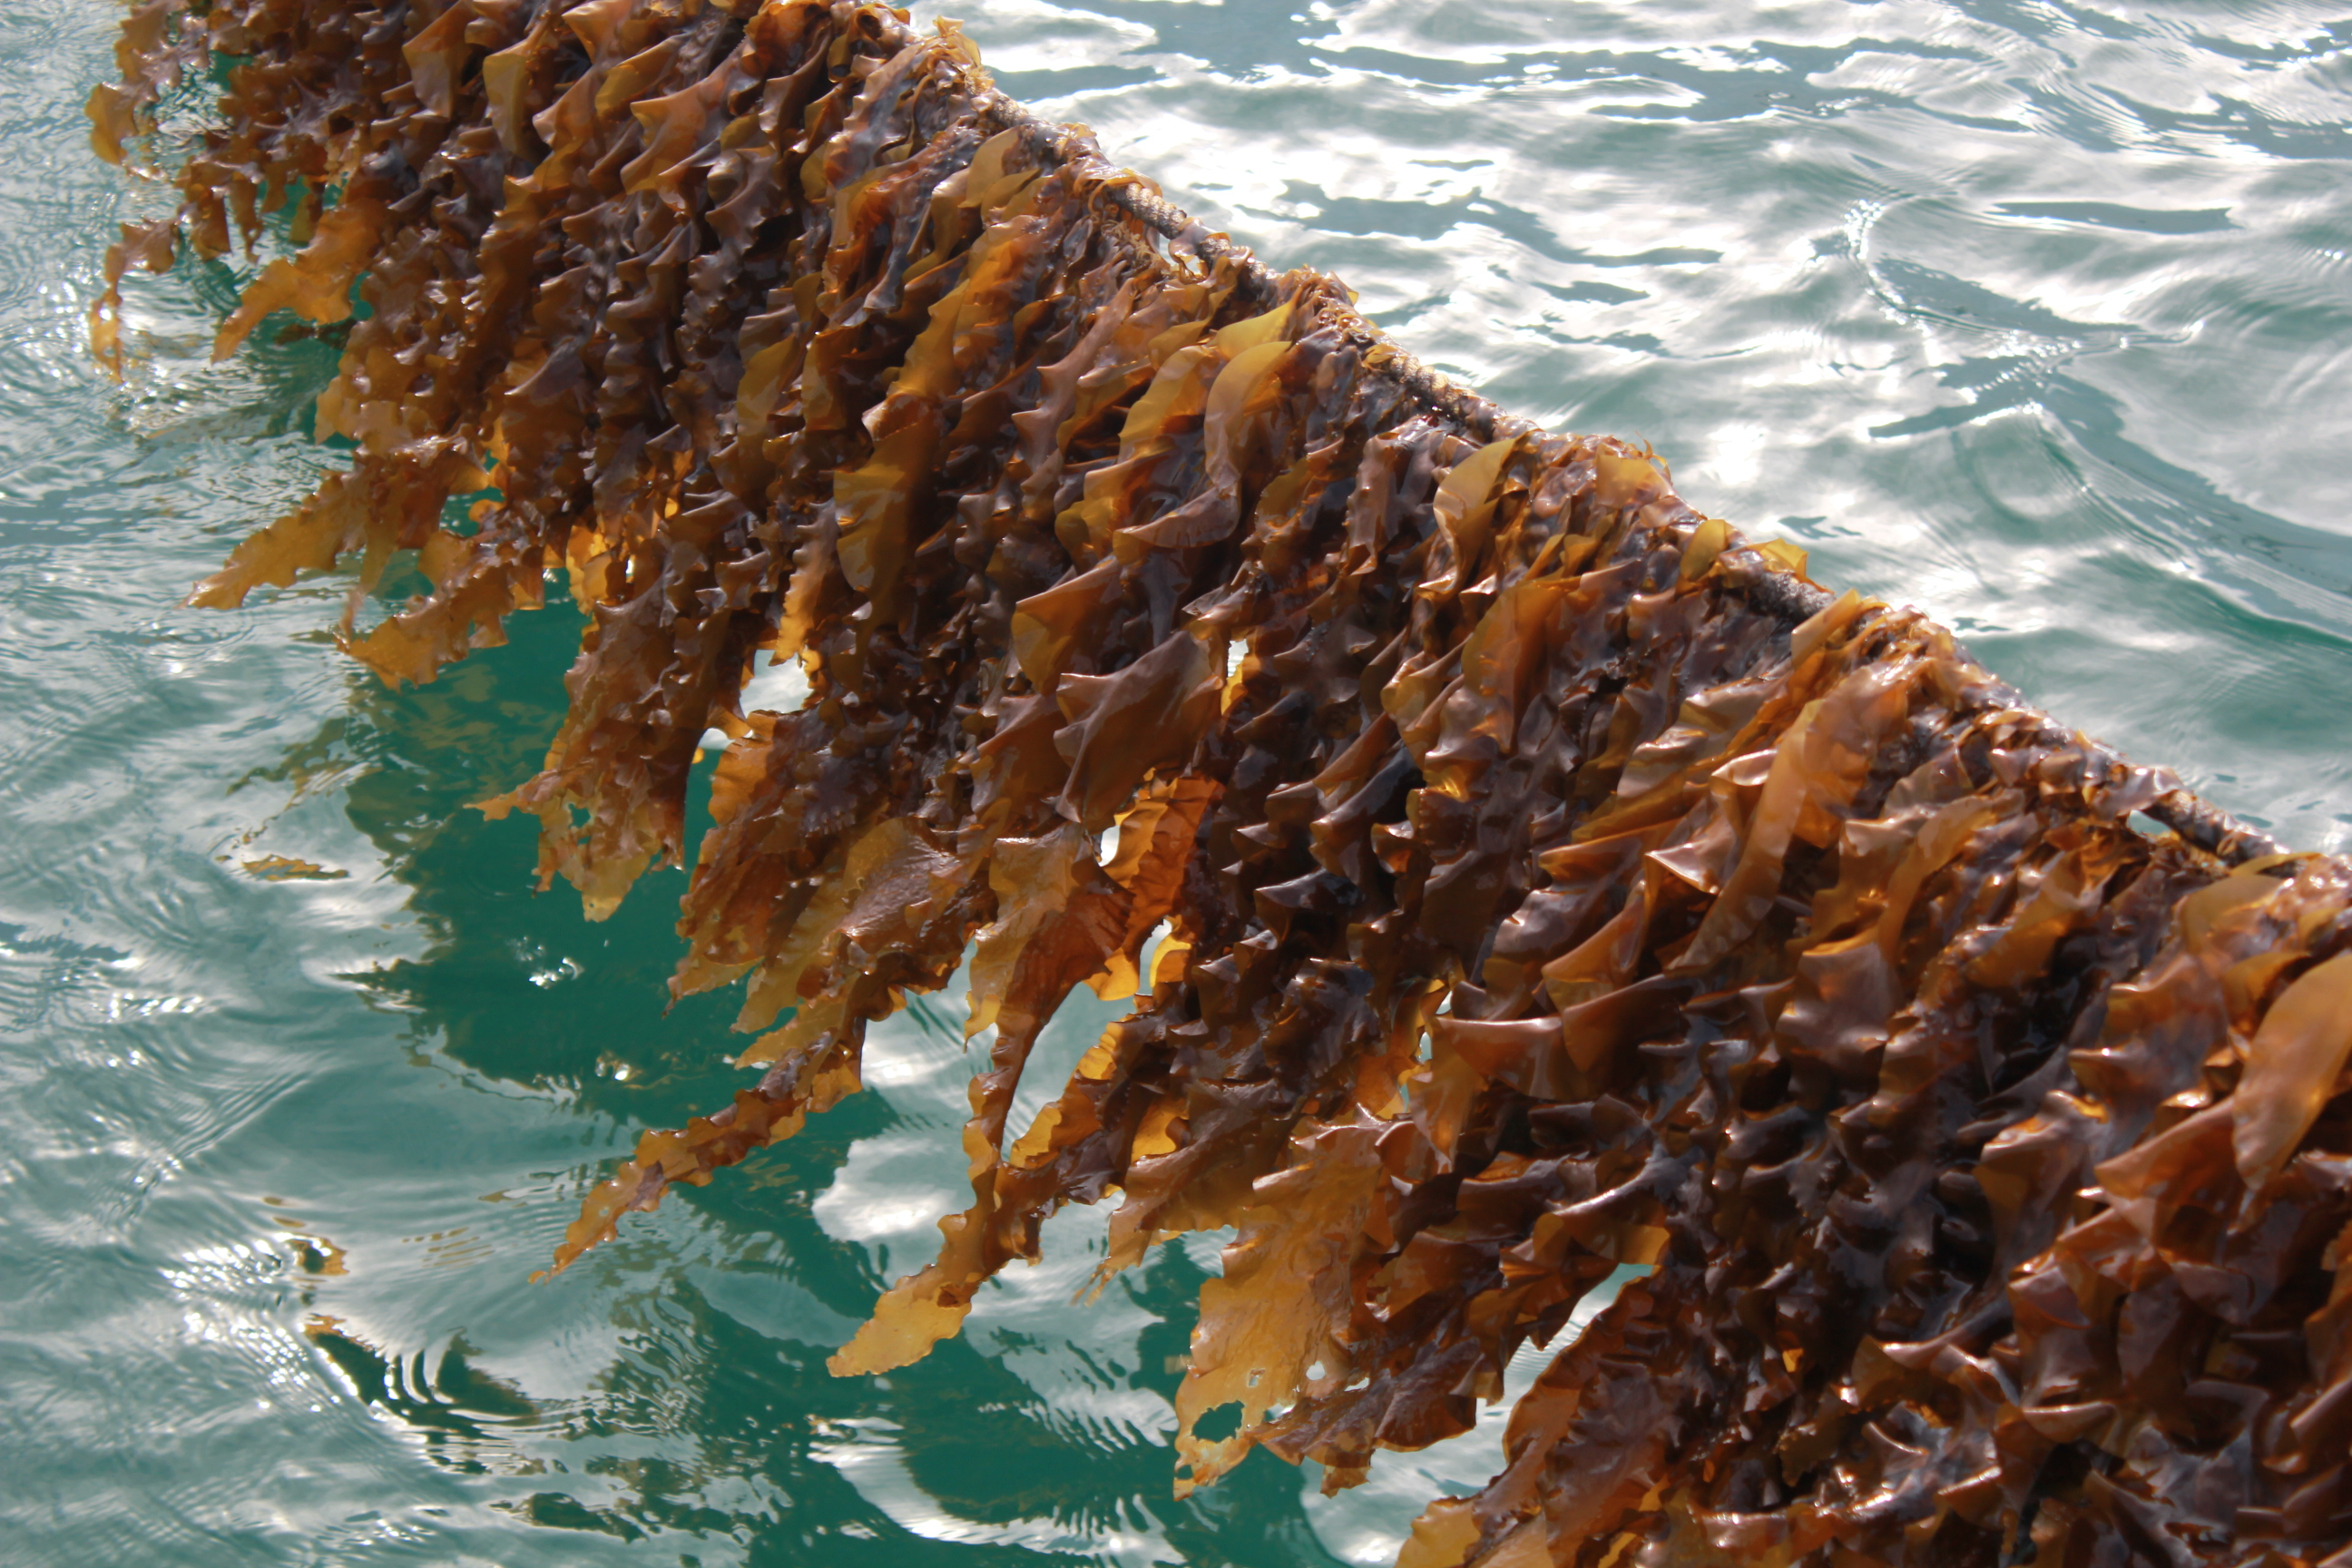
\includegraphics[width=\textwidth]{kelp_photo/kelp_photo1}
  \caption{\textit{Saccharina Latissima} being harvested}
\end{figure}


\section{Background on Kelp Models}

Mathematical modeling of macroalgae growth is not a new topic, although it is a reemerging one.
Several authors in the second half of the twentieth century were interested in describing the growth and composition of the macroalgae \textit{Macrocystis pyrifera}, commonly known as ``giant kelp,'' which grows prolifically off the coast of southern California.
The first such mathematical model was developed by W.J. North for the Kelp Habitat Improvement Project at the California Institute of Technology in 1968 using seven variables.
By 1974, Nick Anderson greatly expanded on North's work, and created the first comprehensive model of kelp growth which he programmed using FORTRAN \cite{anderson_mathematical_1974}.
In his model, he accounts for solar radiation intensity as a function of time of year and time of day, and refraction on the surface of the water.
He uses a simple model for shading, simply specifying a single parameter which determines the percentage of light which is allowed to pass through the kelp canopy floating on the surface of the water.
He also accounts for attenuation due to turbidity using Beer's Law.
Using this data on the availability of light, he calculates the photosynthesis rates and the growth experienced by the kelp. \\[-0.75em]

Over a decade later in 1987, G.A.
Jackson expanded on Anderson's model for \textit{Macrocystis pyrifera}, with an emphasis on including more environmental parameters and a more complete description of the growth and decay of the kelp \cite{jackson_modelling_1987}. 
He takes into account respiration, frond decay, and most importantly for my work, sub-canopy light attenuation due to self-shading.
He simply adds a coefficient to the exponential decay of light as a function of depth to represent shading from kelp fronds.
He doesn't consider and radial nor angular dependence on shading. 
Jackson also expands Anderson's definition of canopy shading, treating the canopy not as a single layer, but as 0, 1, or 2 discrete layers, each composed of individual fronds.
While this is a significant improvement over Anderson's light model, it is still rather simplistic. \\[-0.75em]

Both Anderson's and Jackson's model were carried out by numerically solving a system of differential equations over small time intervals.
In 1990, M.A. Burgman and V.A. Gerard developed a stochastic population model \cite{burgman_stage-structured_1990}.
This approach is quite different, and functions by dividing kelp plants into groups based on size and age, and generating random numbers to determine how the population distribution over these groups changes over time, based on measured rates of growth, death, decay, light availability, etc.
That same year, Nyman et. al. tested a similar model in New Zealand, as well as a Markov chain model, and compared the results with experimental data \cite{nyman_macrocystis_1990}. \\[-0.75em]

In 1996 and 1998 respectively, P. Duarte and J.G. Ferreira used the size-class approach to create a more general model of macroalgae growth, and Yoshimori et. al. created a differential equation model of \textit{Laminaria religiosa} with specific emphasis on temperature dependence of growth rate \cite{duarte_model_1997,yoshimori_mathematical_1998}.
These were the some of the first models of kelp growth that did not specifically relate to \textit{Macrocystis pyrifera} (``giant kelp''). 
Initially, there was a great deal of excitement about this species due to it's incredible size and growth rate, but difficulties in harvesting and negative environmental impacts have caused scientists to investigate other kelp species. \\[-0.75em]

\section{Background on Radiative Transfer}
In terms of optical quantities, our primary interest is in the radiance at each point from all directions, which affects the photosynthetic rate of the kelp, and therefore the total amount of biomass producible in a given area as well as the total nutrient remediation potential.
The equation governing the radiance throughout the system is known as the Radiative Transfer Equation (RTE), which has been largely unutilized in the fields of oceanography and aquaculture.
Meanwhile, it has been studied extensively in two fields: stellar astrophysics and computer graphics.
In its full form, radiance is a function of 3 spatial dimensions, 2 angular dimensions, and frequency, making for an incredibly complex problem.
In this work, frequency is ignored, only monochromatic radiation is considered.
The RTE states that along a given path, radiance is decreased by absorption and scattering out of the path, while it is increased by emission and scattering into the path.
In our situation, emission is negligible, owing only perhaps to some small luminescent phytoplankton or some such anomaly, and can therefore be safely ignored.

We use monochromatic radiative transfer in order to model the light field in an aqueous environment populated by vegetation.
The vegetation (kelp) is modeled by a spatial probability distribution, which we assume to be given.
The two quantities we seek to compute are \textit{radiance} and \textit{irradiance}.
Radiance is the intensity of light in at a particular point in a particular direction, while irradiance is the total light intensity at a point in space, integrated over all angles.
The Radiative Transfer Equation is an integro-partial differential equation for radiance, which has been used primarily in stellar astrophysics; it's application to marine biology is fairly recent \cite{mobley_radiative_2001}.

Understanding the growth rate and nutrient recovery by
kelp cultures has important marine biological implications. For example, recent
work by our research group at Clarkson University, the University of Maine, and
SINTEF Fisheries and Aquaculture is investigating kelp aquaculture as a means to
recover nutrients from wastewater effluent plumes in coastal environments into a
valuable biomass feedstock for many products. Current models for kelp growth
place little emphasis on the way in which nearby plants shade one another.
Self-shading may be a significant model feature, though, as light availability
may impact the growth and composition of the kelp biomass, and thus the mixture
of goods that may be derived.

\section{Overview of Thesis}
The remainder of this document is organized as follows.
In Chapter \ref{chap:kelp}, we develop a probabilistic model to describe the spatial distribution of kelp by assuming simple distributions for the lengths and orientations of fronds.
We begin Chapter \ref{chap:light} with a survey of fundamental radiometric quantities and optical properties of matter.
We use the spatial kelp distribution from Chapter \ref{chap:kelp} to determine optical properties of the combined water-kelp medium.
We then present the Radiative Transfer Equation, an integro-partial differential equation which describes the the light field as a function of position and angle.
An asymptotic expansion is explored for cases where absorption dominates scattering in the medium, such as in very clear water or high kelp density.
In Chapter \ref{chap:numerical}, details are given for the numerical solution of the equations from Chapters \ref{chap:kelp} and \ref{chap:light}.
Both the full finite difference solution and the asymptotic approximation are described.
Next, in Chapter \ref{chap:parameters}, we discuss the availability of necessary parameters in the literature.
For those which are not readily available, we give rough estimates and briefly describe experimental methods for their determination.
Then, in Chapter \ref{chap:model_analysis}, we investigate the necessary grid resolution for adequate accuracy in the full finite difference solution and compare to the asymptotic approximation for a few parameter sets.
Further, we determine the effect of varying a few key parameters on the light field predicted by the asymptotic approximation.
Afterwards, we use the light model developed here in a full lifecycle simulation of kelp growth and compare the light field and biomass production to those predicted by a simpler 1D exponential decay light model.
Finally, we conclude with Chapter \ref{chap:conclusion} by giving a brief summary of the model, discuss and its performance, and suggest improvements and avenues for future work.
 \chapter{KELP MODEL}
\label{chap:kelp}

In order to properly model the spatial distribution of light around the kelp, it is first necessary to formulate a spatial description of the kelp, which we do in this chapter.
We take a probabilistic approach to describing the kelp.
We begin by describing the distribution of kelp fronds, and through algebraic manipulation, we are able to assign to each point in space a probability that kelp occupies the location.

\section{Physical Setup}
Being a salt water species, macroalgae cultivation occurs primarily in the ocean, with the exception of the initial stage of growth, where microscopic kelp spores are inoculated onto a thread in a small laboratory pool.
This thread is then wrapped around a large rope, which is placed in the ocean and generally suspended by buoys in one of two configurations: horizontal or vertical.
Thus far, I am primarily concerned with modeling the vertical rope case, in which the kelp plants extend radially outward from the rope in all directions, which are made up of a single frond (leaf), stipe (stem) and holdfast (root structure).
We consider a rectangular grid of such vertical ropes. 
Plants extending from each rope will shade both themselves and their neighbors
to varying degrees based on the depth of the kelp, the rope spacing, the angle
of incident light on the surface and the nature of scattering in the water.
In addition, light will be naturally absorbed by the water to varying degrees as determined by the clarity of the water.

\begin{figure}[H]
	\centering
	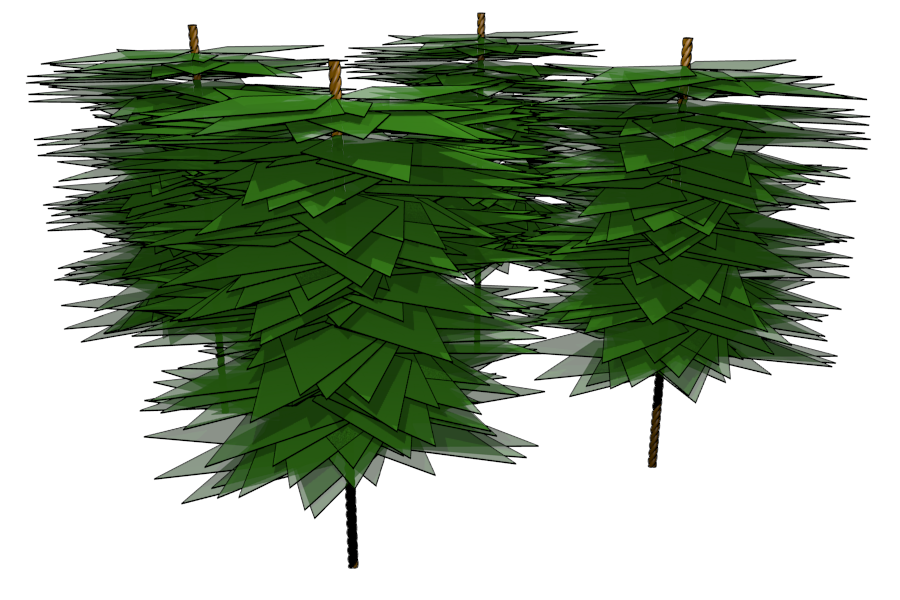
\includegraphics[width=3.5in]{kelp_array}
	\captionof{figure}{$4\times 4$ array of vertical kelp ropes}
\end{figure}
\section{Coordinate System}

Consider the rectangular domain
\begin{align*}
  \xmin &\leq x \leq \xmax, \\
  \ymin &\leq y \leq \ymax, \\
  \zmin &\leq z \leq \zmax.
\end{align*}
For all three dimensional analysis, we use the absolute coordinate system defined in figure \ref{fig:3dcoords}.
In the following sections, it is necessary to convert between Cartesian and spherical coordinates, which we do using the relations
\begin{align}
	\begin{split}
		x & = r\sin\phi\cos\theta, \\
		y & = r\sin\phi\sin\theta, \\
		z & = r\cos\phi. \\
	\label{eqn:coords}
	\end{split}
\end{align}

Therefore, for some function $f(x,y,z)$, we can write its derivative along a path in spherical coordinates in terms of Cartesian coordinates using the chain rule.
\begin{equation}
	\frac{\partial f}{\partial r} 
	=\frac{\partial f}{\partial x}\frac{\partial x}{\partial r} 
	+ \frac{\partial f}{\partial y}\frac{\partial y}{\partial r} 
	+ \frac{\partial f}{\partial z}\frac{\partial z}{\partial r}
\end{equation}
Then, calculating derivatives from \eqref{eqn:coords} yields
\begin{equation}
	\frac{\partial f}{\partial r} 
	=\frac{\partial f}{\partial x}\sin\phi\cos\theta
	+ \frac{\partial f}{\partial y}\sin\phi\sin\theta
	+ \frac{\partial f}{\partial z}\cos\phi.
	\label{eqn:partials}
\end{equation}
\begin{figure}[H]
	\centering
	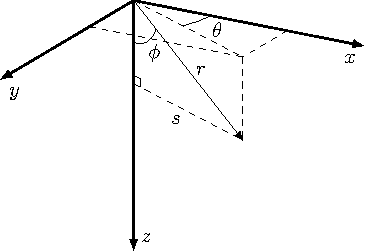
\includegraphics[width=3in]{3d_coords}
	\caption{Downward-facing right-handed coordinate system with radial distance $r$ from the origin, distance $s$ from the $z$ axis, zenith angle $\phi$ and azimuthal angle $\theta$}
	\label{fig:3dcoords}
\end{figure}


\section{Population Distributions}

\subsection{Frond Shape}
\label{sec:shape}


\begin{figure}[h]
	\centering
  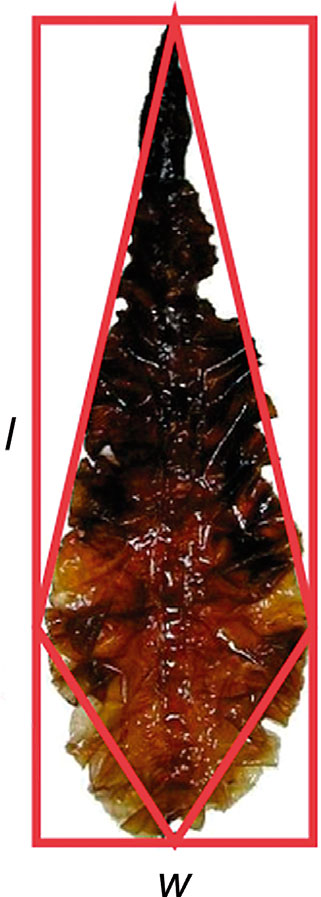
\includegraphics[width=1.2in]{kelp_photo/kite}
  \qquad
	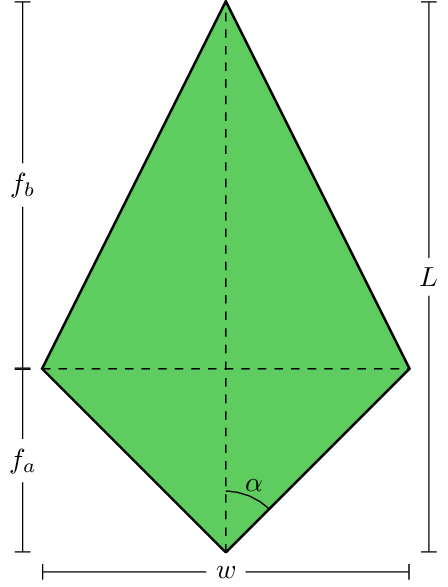
\includegraphics[width=2in]{frond}
	\captionof{figure}{Simplified kite-shaped frond}
	\label{fig:frond}
\end{figure}

We assume the frond is a kite with length $l$ from base to tip, and width $w$ from left to right.
 The shortest distance from the base to the diagonal connecting the left and right corners is called $f_a$, and the shortest distance from that diagonal to the tip is called $f_b$.
 We have
 \begin{equation}
	 f_a + f_b = l
 \end{equation}
When considering a whole population with varying sizes, it is more convenient to specify ratios than absolute lengths.
Let the following ratios be defined.
\begin{align}
	f_r &= \frac{l}{w} \\
	f_s &= \frac{f_a}{f_b}
\end{align}
These ratios are assumed to be consistent among the entire population, making all fronds geometrically similar.
With these definitions, the shape of the frond can be fully specified by $l$, $f_r$, and $f_s$.
It is possible, then, to redefine $w$, $f_a$ and $f_b$ as follows from the preceding formulas.

\begin{align}
	w &= \frac{l}{f_r} \\
	f_a &= \frac{lf_s}{1+f_s} \\
	f_b &= \frac{l}{1+f_s}
\end{align}

The angle $\alpha$, half of the angle at the base corner, is also important in our analysis.
Using the above equations,
\begin{equation}
	\alpha = \tan^{-1}\left(\frac{2f_rf_s}{1+f_s}\right)
\end{equation}

The area of the frond is given by
\begin{equation}
  A = \frac{lw}{2} = \frac{l^2}{2f_r}.
\end{equation}

Likewise, if the area is known, then the length is
\begin{equation}
  l = \sqrt{2Af_r}
  \label{eqn:length-from-area}
\end{equation}

\subsection{Length and Angle Distributions}
\label{sec:dist}
We assume that frond lengths are normally distributed with mean $\mu_l$ and standard deviation $\sigma_l$.
We assume the frond angle varies according to the von Mises distribution, which is the periodic analogue of the normal distribution, defined on $[-\pi,\pi]$ rather than $(-\infty,\infty)$.
The von Mises distribution has two parameters, $\mu$ and $\kappa$, which shift and sharpen its peak respectively, as shown in Figure \ref{fig:vonmises}.
$\kappa$ can be considered analogous to $1/\sigma$ in the normal distribution.
Here, we use $\mu = \theta_w$ and $\kappa = v_w$.
That is, in the case of zero current velocity, the frond angles are be distributed uniformly, while as current velocity increases, they become increasingly likely to be pointing in the direction of the current.
Note that $\theta_w$ and $v_w$ vary over depth.

The PDF for this distribution is
\begin{equation}
	P_{\theta_f}(\theta_f) = \frac{\exp\left(v_w\cos(\theta_f-v_w)\right)}{2\pi I_0(v_w)}
\end{equation}
where $I_0(x)$ is the modified Bessel function of the first kind of order 0.
Notice that unlike the normal distribution, the von Mises distribution approaches a \textit{non-zero} uniform distribution as $\kappa$ approaches 0.
\begin{equation}
	\displaystyle \lim_{v_w \to 0}P_{\theta_f}(\theta_f) = \frac{1}{2\pi} \;\forall\, \theta_f \in [-\pi,\pi]
\end{equation}

\begin{figure}[h]
	\centering
	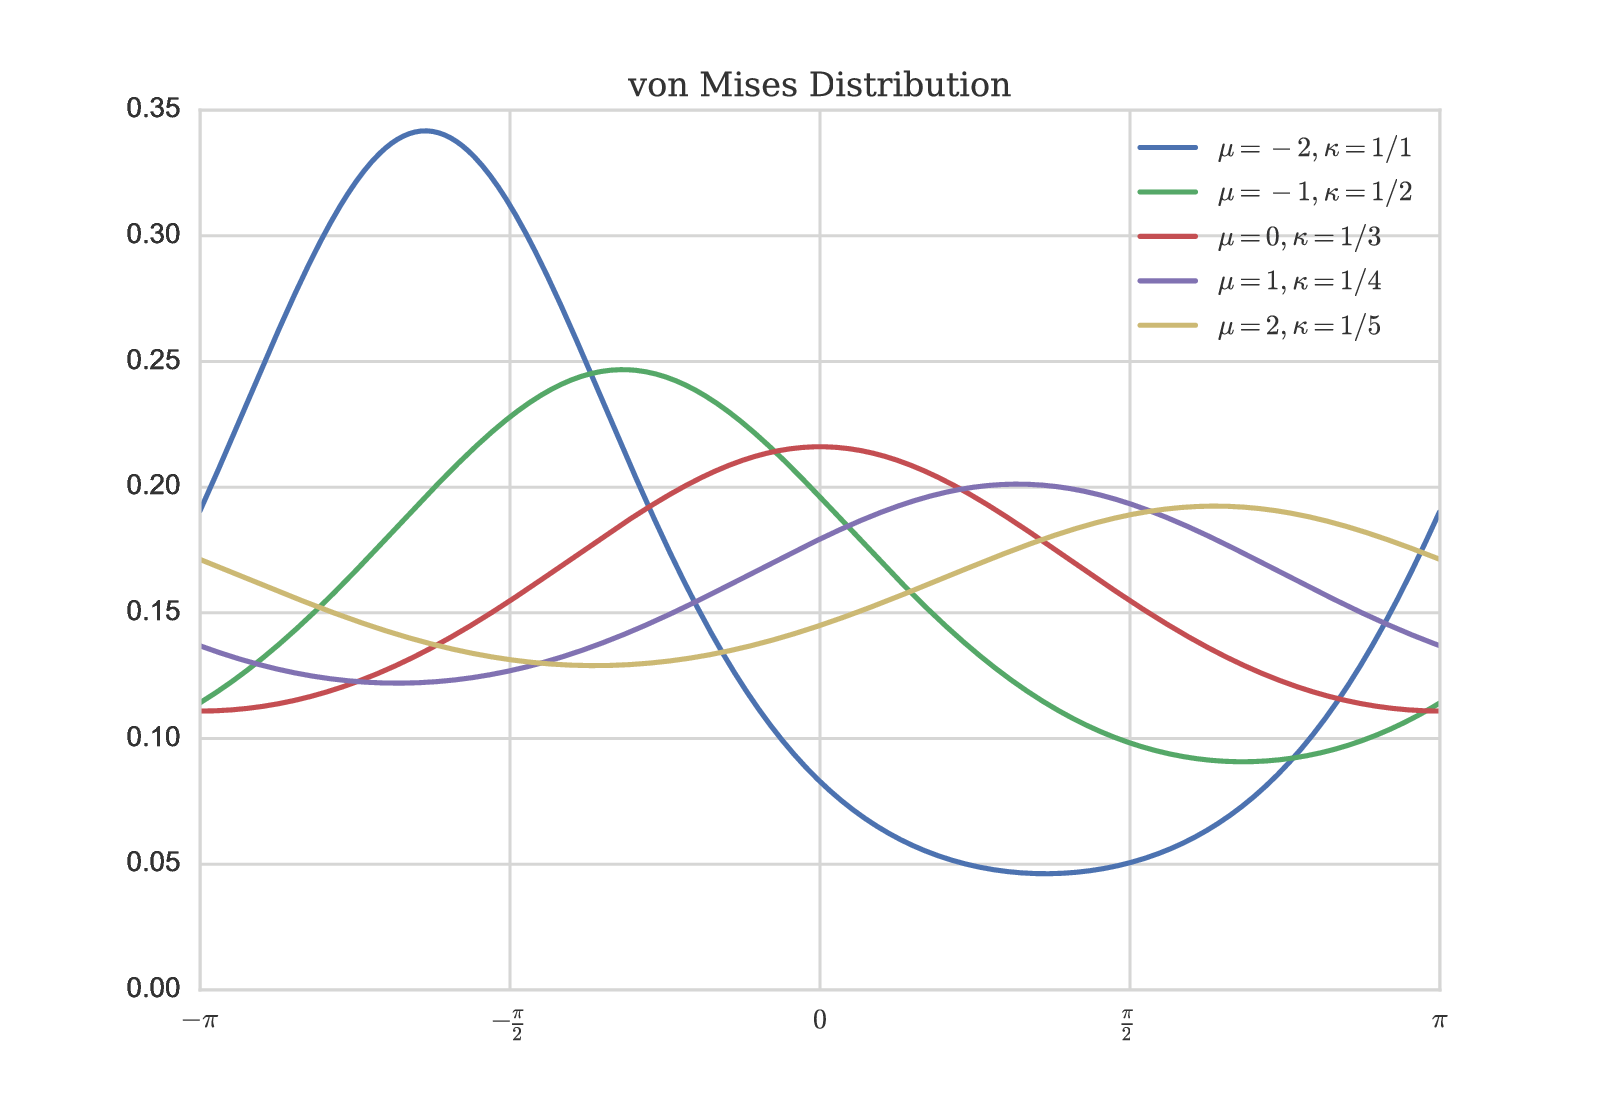
\includegraphics[width=.75\linewidth]{vonmises_2}
	\captionof{figure}{von Mises distribution for a variety of parameters}
	\label{fig:vonmises}
\end{figure}

\subsection{Joint Length-Orientation Distribution}
\label{sec:2d_dist}
The previous two distributions can reasonably be assumed to be independent of one another. That is, the angle of the frond does not depend on the length, or vice versa.
Therefore, the probability of a frond simultaneously having a given frond length and angle is the product of their individual probabilities.

Given independent events $A$ and $B$,
\begin{equation}
	\label{eq:ind_prob}
	P(A \cap B) = P(A)P(B)
\end{equation}
Then the probability of frond length $l$ and frond angle $\theta_f$ coinciding is 
\begin{equation}
	P_{2D}(\theta_f,l) = P_{\theta_f}(\theta_f) \cdot L(l)
\end{equation}
A contour plot of this 2D distribution for a specific set of parameters is shown in figure \ref{fig:dist_2d}, where probability is represented by color in the 2D plane.
Darker green represents higher probability, while lighter beige represents lower probability.
In figure \ref{fig:kelp_sample}, 50 samples are drawn from this distribution and plotted.

It is important to note that if $P_{\theta_f}$ were dependent on $l$, the above definition of $P_{2D}$ would no longer be valid.
For example, it might be more realistic to say that larger fronds are less likely to bend towards the direction of the current.
In this case, \eqref{eq:ind_prob} would no longer hold, and it would be necessary to use the following more general relation.
\begin{equation}
	P(A \cap B) = P(A)P(B|A) = P(B)P(B|A)
\end{equation}
This is currently not taken into consideration in this model.

\begin{figure}[h]
	\centering
	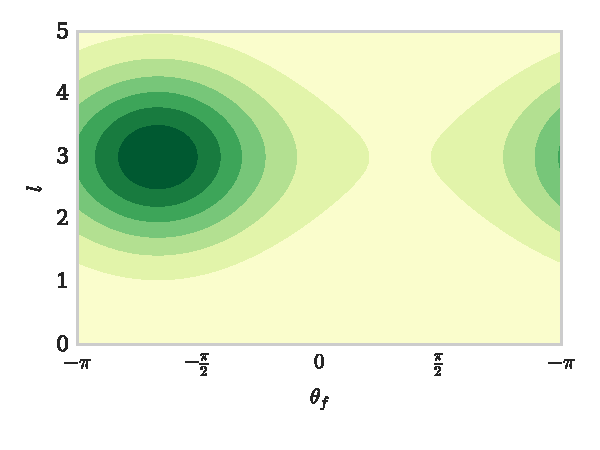
\includegraphics[width=.75\linewidth]{prob_2d}
	\vspace{-3em}
	\captionof{figure}{2D length-angle probability distribution with $\theta_w=2\pi/3,v_w=1$}
	\label{fig:dist_2d}
\end{figure}

\begin{figure}[h]
	\centering
	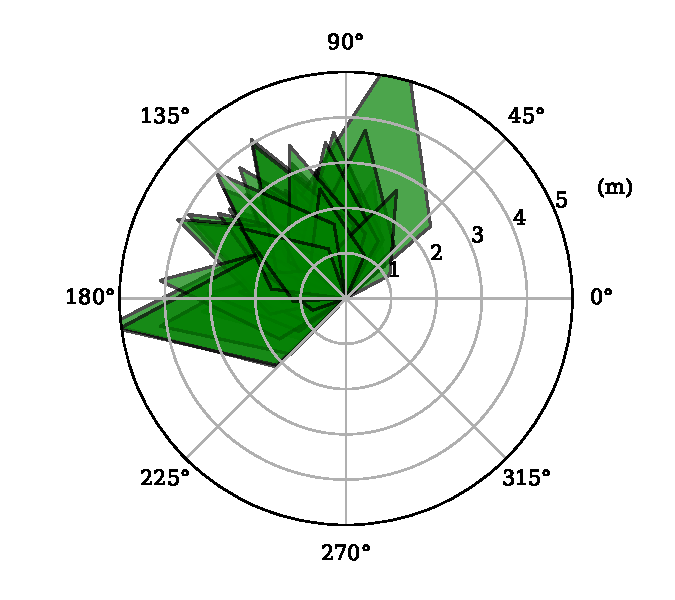
\includegraphics[width=.75\linewidth]{kelp_sample}
	\vspace{-2em}
	\captionof{figure}{A sample of 50 kelp fronds with length and angle picked from the distribution above with $f_s=0.5$ and $f_r=2$.}
	\label{fig:kelp_sample}
\end{figure}

\section{Spatial Distribution}
\subsection{Rotated Coordinate System}
\label{sec:rot_coords}
To determine under what conditions a frond will occupy a given point, we begin by
describing the shape of the frond in Cartesian and then converting to polar coordinates.
Of primary interest are the edges connected to the frond tip.
For convenience, we will use a rotated coordinate system $(\theta',s)$ such that the line connecting the base to the tip is vertical, with the base at $(0,0)$.
The Cartesian analogue of this coordinate system, $(x',y')$, has the following properties.
\begin{align}
	x' &= s\cos\theta' \\ 
	y' &= s\sin\theta'
\end{align}
and
\begin{align}
	s &= \sqrt{x'^2+y'^2}
\end{align}
\vspace{-1em}
\begin{align}
	\theta' &= \atantwo(y, x)
\end{align}

\subsection{Functional Description of Frond Edge}
With this coordinate system established, we can describe the outer two edges of the frond in Cartesian coordinates as a piecewise linear function connecting the left corner: $(-w/2,f_a)$, the tip: $(0,l)$, and the right corner: $(w/2,f_a)$.
This function has the form
\begin{equation}
	y'_f(x') = l-\sign(x')\frac{f_b}{w/2}x'.
\end{equation}

Using the equations in Section \ref{sec:rot_coords}, this can be written in polar coordinates after some rearrangement as
\begin{equation}
	s_f'(\theta') = \frac{l}{\sin\theta' + S(\theta')\frac{2f_b}{w}\cos\theta'}
\end{equation}
where
\begin{equation}
	S(\theta') = \sign(\theta'-\pi/2)
\end{equation}

Then, using the relationships in Section \ref{sec:shape}, we can rewrite the above equation in terms of our frond ratios $f_s$ and $f_r$.
\begin{equation}
	\label{eq:rf_rel}
	s_f'(\theta') = \frac{l}{\sin\theta' + S(\theta')\frac{2f_r}{1+f_s}\cos\theta'}
\end{equation}

\subsection{Absolute Coordinates}
\label{sec:abs_coords}
To generalize to a frond pointed at an angle $\theta_f$, we will use the coordinate system $(\theta,s)$ such that
\begin{equation}
	\theta = \theta' + \theta_f - \frac{\pi}{2}
\end{equation}
Then, for a frond pointed at the arbitrary angle $\theta_f$, the function for the outer edges can be written as 
\begin{equation}
	\label{eq:rf_abs}
	s_f(\theta) = s_f'\left(\theta - \theta_f + \frac{\pi}{2} \right)
\end{equation}


\subsection{Conditions for Occupancy}
Consider a fixed frond of length $l$ at an angle $\theta_f$. The point
$(\theta,s)$ is occupied by the frond if
\begin{align}
	\left|\theta_f - \theta \right| < \alpha
	\shortintertext{and}
	s < s_f(\theta)
\end{align}

Equivalently, letting the point $(\theta,s)$ be fixed, a frond occupies the point if the following conditions are satisfied.
\begin{align}
	\theta - \alpha < \theta_f < \theta + \alpha
	\label{eqn:rs_th}
	\shortintertext{and}
	l > l_{min}(\theta,s)
	\label{eqn:rs_l}
\end{align}
where
\begin{equation}
	l_{min}(\theta,s) = s \cdot \frac{l}{s_f(\theta)}
\end{equation}


Then, considering the point to be fixed, \eqref{eqn:rs_th} and \eqref{eqn:rs_l} define the spacial region $R_s(\theta,s)$ called the ``occupancy region for $(\theta,s)$'' with the property that if the tip of a frond lies within this region (i.e. $(\theta_f,l) \in R_s(\theta,s)$), then it occupies the point.
$R_s(3\pi/4,3/2)$ is shown in blue in figure \ref{fig:shade_area} and the smallest possible occupying fronds for several values of $\theta_f$ are shown in various colors.
Any frond longer than these at the same angle will also occupy the point.

\begin{figure}[h]
	\centering
	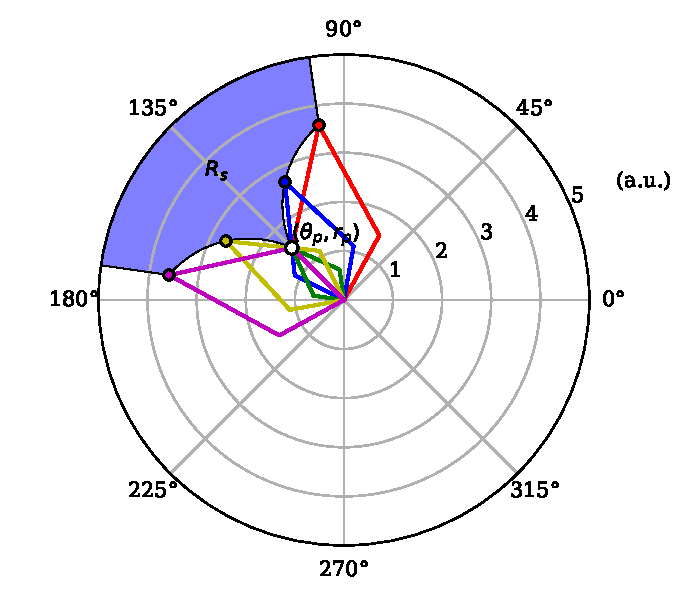
\includegraphics[width=.75\linewidth]{shade_area}
	\vspace{-2em}
	\captionof{figure}{Outlines of minimum-length fronds for a variety of angles to occupy the point $(\theta,s)=(3\pi/4,3/2)$}
	\label{fig:shade_area}
\end{figure}

\subsection{Probability of Occupancy}
We are interested in the probability that, given a fixed point $(\theta,s)$, values of $l$ and $\theta_f$ chosen from the distributions described in Section \ref{sec:dist} will fall in the occupancy region.
This is found by integrating $P_{2D}$ over the occupancy region for $(\theta,s)$, as depicted in figure \ref{fig:cart_shade}.

\begin{figure}[H]
	\centering
	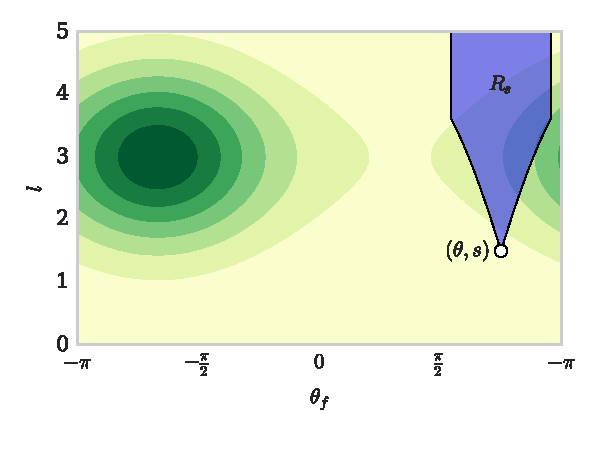
\includegraphics[width=.75\linewidth]{cart_shade}
	\vspace{-3em}
	\captionof{figure}{Contour plot of $P_{2D}(\theta_f,l)$ overlayed with the
    region in the $\theta_f-l$ plane which results in a frond occupying the point $(\theta,s)=(3\pi/4,3/2)$}
	\label{fig:cart_shade}
\end{figure}

Now, integrating $P_{2D}(\theta_f,l)$ over $R_s(\theta,s)$ yields the proportion of the population occupying the point $(\theta,s)$.
\begin{align}
		\tilde{P}_k(\theta,s,z)	&= \iint_{R_s(\theta,s)}
								P_{2D}(\theta_f,l)
								\,dl\,d\theta_f \nonumber \\
							&= \int_{\theta-\alpha}^{\theta+\alpha} 
								\int_{l_{min}(\theta_f)}^\infty
								P_{2D}(\theta_f,l)
								\,dl\,d\theta_f
\end{align}

Then, multiplying $\tilde{P}_k$ by the number of fronds in the population $n$ of the depth layer gives the expected number of fronds occupying the point.
Now, assuming a uniform thickness $t$ for all fronds, and a thickness $dz$ of the depth layer, we find the proportion of the grid cell occupied by kelp to be
\begin{equation}
  P_k = \frac{nt}{dz}\tilde{P}.
\end{equation}

Then, the effective absorption coefficient can be calculated at any point in space as
\begin{equation}
  a(\vec{x}) = P_k(\vec{x})a_k + (1-P_k(\vec{x}))a_w
\end{equation}

\begin{figure}[h]
	\centering
	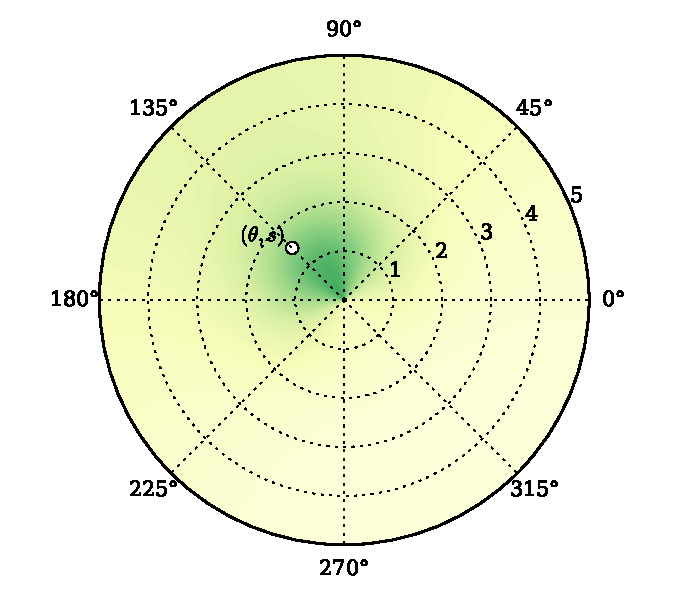
\includegraphics[width=.75\linewidth]{prob_shade}
	\vspace{-2em}
	\captionof{figure}{Contour plot of the probability of occupying sampled at 121 points using $\theta_f=2\pi/3,v_w=1$}
	\label{fig:prob_shade}
\end{figure}
 \chapter{LIGHT MODEL}
\label{chap:light}

Now that we have formulated the distribution of kelp throughout the medium, we introduce the radiative transfer equation, which is used to calculate the light field.

\section{Optical Definitions}

\subsection{Radiometric Quantities}

One of the most fundamental quantities in optics is radiant flux $\Phi$, which is the has units of energy per time.
The quantity of primary interest in modeling the light field is radiance $L$, which is defined as the radiant flux per steradian per projected surface area perpendicular to the direction of propagation of the beam.
That is,

\begin{equation}
	L = \frac{d^2\Phi}{dA d\omega}
\end{equation}

Once the radiance $L$ is calculated everywhere, the irradiance is
\begin{equation}
  I(\vec{x}) = \int_{4\pi}L(\vec{x},\vec{\omega})\, d\omega.
\end{equation}
Integrating $I(\vec{x})$, which has units \SI{}{\W/m^2}, over the surface of a frond, produces the power (with units \SI{}{\W}) transmitted to the frond.
This is discussed further in Section \ref{sec:perceived_irrad}

Irradiance can be converted to moles of photons (also called Einsteins) per second as
\begin{equation}
  \SI{1}{\W\per\m^2} = \SI{4.2}{\micro\mole \,photons\per\second}.
\end{equation}


\subsection{Inherent Optical Properties}
We must now define a few inherent optical properties (IOPs) which depend only on the medium of propagation.
These phenomena are governed by three inherent optical properties (IOPs) of the
medium.
The absorption coefficient $a(\vec{x})$ (units m$^{-1}$) defines the
proportional loss of radiance per unit length.
The scattering coefficient $b$ (units m$^{-1}$), defines the proportional loss
of radiance per unit length, and is assumed to be constant over space.

The volume scattering function (VSF) $\beta(\Delta): [-1, 1] \to \RR^+$ (units sr$^{-1}$) defines the probability of light scattering at any given angle from its source.
Formally, given two directions $\vec{\omega}$ and $\vec{\omega}'$, $\beta(\vec{\omega} \cdot \vec{\omega}')$ is the probability density of light scattering from $\vec{\omega}$ into $\vec{\omega}'$ (or vice-versa).
Of course, since a single direction subtends no solid angle, the probability of scattering occurring exactly from $\vec{\omega}$ to $\vec{\omega}'$ is 0.
Rather, we say that the probability of radiance being scattered from a direction $\omega$ into an element of solid angle $\Omega$ is $\int_\Omega \beta(\vec{\omega} \cdot \vec{\omega}')\, d\vec{\omega}'$.

The VSF is normalized such that
\begin{equation}
  \int_{-1}^1\beta(\Delta)\, d\Delta=\frac{1}{2\pi},
\end{equation}
so that for any $\omega$,
\begin{equation}
  \int_{4\pi}\beta(\vec{\omega}\cdot\vec{\omega}')\, d\vec{\omega}' = 1.
\end{equation}
i.e., the probability of light being scattered to some direction on the unit sphere is 1.


\section{The Radiative Transfer Equation}

\subsection{Ray Notation}
Consider a fixed position $\vec{x}$ and direction $\vec{\omega}$ such that
$\vec{\omega} \cdot \hat{z} \neq 0$.


Let $\vec{l}(\vec{x}, \vec{\omega}, s)$ denote the linear path containing $\vec{x}$
with initial z coordinate given by
\begin{equation}
  z_0 =
   \begin{cases}
    0, & \vec{\omega} \cdot \hat{z} < 0 \\
    \zmax, & \vec{\omega} \cdot \hat{z} > 0
  \end{cases}
\end{equation}

Then,
\begin{equation}
  \vec{l}(\vec{x}, \vec{\omega}, s) = \frac{1}{\tilde{s}} (s\vec{x} + (\tilde{s} - s)\vec{x_0}(\vec{x}, \vec{\omega}))
\end{equation}

where
\begin{equation}
  \vec{x_0}(\vec{x}, \vec{\omega}) = \vec{x} - \tilde{s} \vec{\omega}
\end{equation}
is the origin of the ray, and 

\begin{equation}
  \tilde{s} = \frac{\vec{x} \cdot \hat{z} - z_0}{\vec{\omega} \cdot \hat{z}}
\end{equation}
is the path length from $\vec{x_0}(\vec{x}, \vec{\omega})$ to $\vec{x}$.

\subsection{Colloquial Description}
Denote the radiance at $\vec{x}$ in the direction $\vec{\omega}$ by $L(\vec{x}, \vec{\omega})$.
As light travels along $\vec{l}(\vec{x}, \vec{\omega}, s)$, interaction with the
medium produces three phenomena of interest:
\begin{enumerate}
  \item Radiance is decreased due to absorption.
  \item Radiance is decreased due to scattering out of the path to other
    directions.
  \item Radiance is increased due to scattering into the path from other
      directions.
\end{enumerate}

\subsection{Equation of Transfer}
Then, combining these phenomena, the Radiative Transfer equation along
$\vec{l}(\vec{x}, \vec{\omega})$ becomes
\begin{equation}
  \label{eqn:rte1d}
  \frac{dL}{ds}(\vec{l}(\vec{x}, \vec{\omega}, s), \vec{\omega})
  = -(a(\vec{x}) + b)L(\vec{x}, \vec{\omega})
  + b \int_{4\pi} \beta(\vec{\omega}\cdot\vec{\omega}') L(\vec{x})\, d\omega',
\end{equation}
where $\int_{4\pi}$ denotes integration over the unit sphere.

Now, we have
\begin{align*}
  \frac{dL}{ds}(\vec{l}(\vec{x}, \vec{\omega}, s), \vec{\omega})
    &= \frac{d\vec{l}}{ds}(\vec{x}, \vec{\omega}, s) \cdot \nabla L(\vec{x}, \vec{\omega}', \vec{\omega}) \\
    &= \vec{\omega} \cdot \nabla L(\vec{x}, \vec{\omega})
\end{align*}

Then, the general form of the Radiative Transfer Equation is
\begin{equation}
  \vec{\omega} \cdot \nabla L(\vec{x}, \vec{\omega})
  = -(a(\vec{x}) + b)L(\vec{x}, \vec{\omega})
  + b \int_{4\pi} \beta(\vec{\omega}\cdot\vec{\omega}') L(\vec{x}, \vec{\omega}')\, d\omega'
\end{equation}

or, equivalently,
\begin{equation}
  \vec{\omega} \cdot \nabla L(\vec{x}, \vec{\omega})
  + a(\vec{x})L(\vec{x}, \vec{\omega})
  = b \left(
    \int_{4\pi} \beta(\vec{\omega}\cdot\vec{\omega}') L(\vec{x}, \vec{\omega}')\, d\omega'
    - L(\vec{x}, \vec{\omega})
  \right)
\end{equation}

\subsection{Boundary Conditions}

We use periodic boundary conditions in the $x$ and $y$ directions.
\begin{align}
  L\left((\xmin, y, z), \vec{\omega}\right) &= L\left((\xmax, y, z), \vec{\omega}\right) \\
  L\left((x, \ymin, z), \vec{\omega}\right) &= L\left((x, \ymax, z), \vec{\omega}\right)
\end{align}

In the $z$ direction, we specify a spatially uniform downwelling light just
under the surface of the water by a function $f(\vec{\omega})$.
Or if $\zmin>0$, then the radiance at $z=\zmin$ should be specified instead (as opposed to the radiance at the first grid cell center).

Further, we assume that no upwelling light enters the domain from the bottom.
\begin{align}
  L(\vec{x_s}, \vec{\omega}) &= f(\omega) \mbox{ if } \vec{\omega} \cdot \hat{z} > 0\\ 
  L(\vec{x_b}, \vec{\omega}) &= 0 \mbox { if } \vec{\omega} \cdot \hat{z} < 0
\end{align}
 
\section{Low-Scattering Approximation}
In clear waters where absorption is more important than scattering, an asymptotic expansion can be used whereby the light field is generated through a sequence of discrete scattering events.
\subsection{Asymptotic Expansion}
Taking $b$ to be small, we introduce the asymptotic series
\newcommand{\Lasym}{L_0(\vec{x},\vec{\omega}) + b L_1(\vec{x},\vec{\omega}) + b^2 L_2(\vec{x},\vec{\omega}) + \cdots}
\newcommand{\Lasyms}{L_0(\vec{x_s},\vec{\omega}) + b L_1(\vec{x_s},\vec{\omega}) + b^2 L_2(\vec{x_s},\vec{\omega}) + \cdots}
\newcommand{\Lasymp}{L_0(\vec{x},\vec{\omega}') + b L_1(\vec{x},\vec{\omega}') + b^2 L_2(\vec{x},\vec{\omega}') + \cdots}
\begin{align}
  L(\vec{x},\vec{\omega}) = \Lasym.
\end{align}
Then, substituting the above into the RTE,
\begin{equation}
  \begin{split}
    &\vec{\omega} \cdot \nabla \left[ \Lasym \right] \\
    &+ a(\vec{x}) \left[ \Lasym \right] \\
    &= b\Bigg(
      \int_{4\pi} \beta(\abs{\vec{\omega} - \vec{\omega}'})
      \left[ \Lasymp \right] \, d\vec{\omega}' \\
    &- \left[ \Lasym \right]
    \Bigg)
    \end{split}
\end{equation}
Then, grouping like powers of $b$, we have the decoupled set of equations
\begin{align}
  \vec{\omega} \cdot \nabla L_0(\vec{x}, \vec{\omega}) + a(\vec{x})L_0(\vec{x}) &= 0 \\
  \vec{\omega} \cdot \nabla L_1(\vec{x}, \vec{\omega}) + a(\vec{x})L_1(\vec{x})
  &= \int_{4\pi} \beta(\abs{\vec{\omega} - \vec{\omega}'}) L_0(\vec{x}, \vec{\omega}')\,d\vec{\omega}' - L_0(\vec{x}, \vec{\omega}) \\ 
  \vec{\omega} \cdot \nabla L_2(\vec{x}, \vec{\omega}) + a(\vec{x})L_2(\vec{x})
  &= \int_{4\pi} \beta(\abs{\vec{\omega} - \vec{\omega}'}) L_1(\vec{x}, \vec{\omega}')\,d\vec{\omega}' - L_1(\vec{x}, \vec{\omega}) \\ 
  &\vdots \nonumber
\end{align}

For boundary conditions, let $x_s$ be a point on the surface of the domain.
Then, 
\begin{equation}
  \Lasyms =
  \begin{cases}
    f(\omega), & \hat{z}\cdot\omega > 0 \\
    0, & \mbox{otherwise},
  \end{cases}
\end{equation}
which becomes
\begin{align}
  L_0(\vec{x}, \vec{\omega}) &=
  \begin{cases}
    f(\omega), & \hat{z}\cdot\omega > 0, \\
    0, & \mbox{otherwise},
  \end{cases} \\
  L_1(\vec{x}, \vec{\omega}) &= 0 \\
  L_2(\vec{x}, \vec{\omega}) &= 0. \\
  &\vdots \nonumber
\end{align}

 
\subsection{Analytical Solution}
\label{sec:asymptotic_sol}

For all $\vec{x}, \vec{\omega}$, let
\begin{align}
  \tilde{a}(s) &= a(\vec{l}(\vec{x}, \vec{\omega}), s), \\ 
  \frac{du_0}{ds}(s) + \tilde{a}(s) u_0(s) &= 0, u_0(0) = f(\vec{\omega})
\end{align}
Then,
\begin{align}
  u_0(s) = f(\omega) \exp\left(-\int_0^s \tilde{a}(s)\, ds\right), \\
  L_0(\vec{l}(\vec{x}, \vec{\omega},s), \vec{\omega}) = u_0(s)
\end{align}

\begin{align}
  g_n(s) = \int_{4\pi} \beta(\abs{\vec{\omega} - \vec{\omega}'})
  L_{n-1}(\vec{l}(\vec{x}, \vec{\omega'}, s), \vec{\omega}')\,d\vec{\omega}' - L_{n-1}(\vec{l}(\vec{x}, \vec{\omega}, s), \vec{\omega}) \\ 
  \frac{du_n}{ds}(s) + \tilde{a}(s)u_n(s) = g_n(s), u_n(0) = 0
\end{align}

Then,
\begin{align}
  u_n(s) = \int_0^sg_n(s')\exp\left( -\int_{s''}^{s'}\tilde{a}(s'')\,ds'' \right)\, ds' \\
  L_n(\vec{l}(\vec{x}, \vec{\omega}, s), \vec{\omega}) = u_n(s)
\end{align}
 \chapter{NUMERICAL SOLUTION}
\label{chap:numerical}

In this chapter, the mathematical details involved in the numerical solution of the previously described equations are presented.
It is assumed that this model is run in conjunction with a model describing the growth of kelp over its life cycle, which calls this light model periodically to update the light field.

\section{Super-Individuals}

The algorithm described in this chapter has two components.
First, a probabilistic description of the kelp is generated at each point in a discrete spatial grid.
Second, optical properties of the resulting kelp-water medium are derived, and the light field is calculated.
The first component is described here.

\subsection{Frond Length Distribution}

Rather than model each kelp frond, a subset of the population, called super-individuals, are modelled explicitly, and are considered to represent many identical individuals, as in \citep{scheffer_super-individuals_1994}.
Specifically, at each depth $k$, there are $n$ super-individuals, indexed by $i$.
Super-individual $i$ has a frond area $A_{ki}$ and represents $n_{ki}$ individual fronds.

From \eqref{eqn:length-from-area}, the frond length of the super-individual is $l_{ki} = \sqrt{2A_{ki}f_r}$.
Given the super-individual data, we calculate the mean $\mu$ and standard deviation $\sigma$ frond
lengths using the formulas:
\begin{equation}
  \mu_k = \frac{\ds \sum_{i=1}^N l_{ki}}{\ds \sum_{i=1}^N n_{ki}},
\end{equation}
\begin{equation}
  \sigma_k = \frac{\ds \sum_{i=1}^N \left( l_{ki} - \mu_k \right)^2}{\ds \sum_{i=1}^N n_{ki}}.
\end{equation}
We then assume that frond lengths are normally distributed in each depth layer
with mean $\mu_k$ and standard deviation $\sigma_k$.

\section{Discrete Grid}
The following is a description of the uniform, rectangular spatial-angular grid used
in the numerical implementation of this model.
It is assumed that all simulated quantities are constant over the interior of a
grid cell.

The number of grid cells in each dimension are denoted by $n_x$, $n_y$, $n_z$,
$n_\theta$, and $n_\phi$, with uniform spacings $dx$, $dy$, $dz$, $d\theta$, and
$d\phi$ between adjacent grid points.

The following indices are assigned to each dimension:
\begin{align}
  x &\to i \\
  y &\to j \\
  z &\to k \\
  \theta &\to l \\
  \phi &\to m
\end{align}

It is convenient, however, to use a single index $p$ to refer to directions $\vec{\omega}$ rather than referring to $\theta$ and $\phi$ separately.
Then, the center of a generic grid cell will be denoted as
$(x_i, y_j, z_k, \vec{\omega}_p)$, and the boundaries between adjacent grid cells
will be referred to as \textit{edges}.
One-indexing is employed throughout this document.

\subsection{Spatial Grid}
\begin{figure}[H]
  \centering
  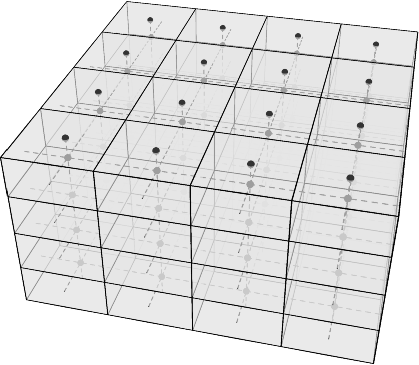
\includegraphics[width=8cm]{spatialgrid.pdf}
  \caption{Spatial grid}
  \label{fig:spatial_grid}
\end{figure}

\begin{align}
  dx &= \frac{x_{\max}-x_{\min}}{n_x} \\ 
  dy &= \frac{y_{\max}-y_{\min}}{n_y} \\ 
  dz &= \frac{z_{\max}-z_{\min}}{n_z}
\end{align}

Denote the edges as 
\begin{align}
  x_i^e &= (i-1)x \mbox{ for } i=1,\ldots,n_x \\
  y_j^e &= (j-1)y \mbox{ for } j=1,\ldots,n_y \\
  z_k^e &= (k-1)z \mbox{ for } k=1,\ldots,n_z 
\end{align}

and the cell centers as
\begin{align}
  x_i &= (i-1/2)dx \mbox{ for } i=1,\ldots,n_x \\
  y_j &= (j-1/2)dy \mbox{ for } j=1,\ldots,n_y \\
  z_k &= (k-1/2)dz \mbox{ for } k=1,\ldots,n_z
\end{align}

Note that in this convention, there are the same number of edges and cells,
and edges preceed centers.

Also, note that no grid center is located on the plane $z=0$.
The surface radiance boundary condition is treated separately.

\subsection{Angular Grid}
\begin{figure}[H]
  \centering
  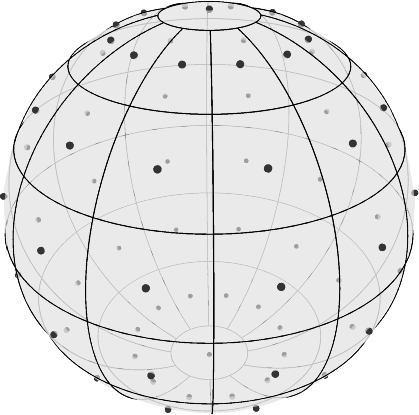
\includegraphics[width=8cm]{angulargrid.pdf}
  \caption{Angular grid at each point in space}
  \label{fig:angular_grid}
\end{figure}

Now, we define the azimuthal angle such that
\begin{align}
  \theta_l = (l-1)d\theta.
\end{align}
For the sake of periodicity, we need
\begin{align}
  \theta_1 &= 0, \\
  \theta_{n_\theta} &= 2\pi-d\theta,
\end{align}
which requires
\begin{equation}
  d\theta = \frac{2\pi}{n_\theta}.
\end{equation}

For the polar angle, we similarly let
\begin{equation}
  \phi_m = (m-1)d\phi
\end{equation}

Since the polar azimuthal is not periodic, we also store the endpoint, so
\begin{align}
  \phi_1 &= 0, \\
  \phi_{n_\phi} &= \pi.
\end{align}

This gives us
\begin{align}
  d\phi &= \frac{\pi}{n_\phi-1}.
\end{align}

It is also useful to define the edges between angular grid cells as
\begin{alignat}{3}
  \theta_l^e &= (l-1/2) d\theta, &\quad l&=1,\ldots,n_\theta \\
  \phi_m^e &= (m-1/2) d\phi, &\quad m&=1,\ldots,n_\phi-1.
\end{alignat}

Note that while $\theta$ has its final edge following its final center, this is
not the case for $\phi$.

\begin{figure}[h]
  \centering
  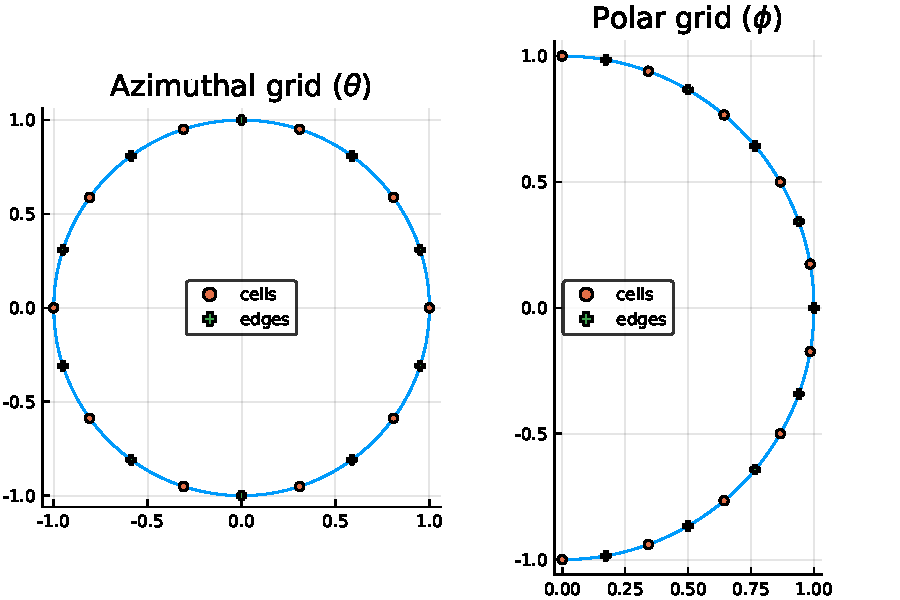
\includegraphics[width=.75\linewidth]{angular_grid_plots}
  \caption{Angular grid}
\end{figure}

As shown in Figure \ref{fig:angular_grid}, $\phi=0$ and $\phi=\pi$, called
the north ($+z$) and south ($-z$) poles respectively, are treated separately.
The total number of angles considered is $n_{\vec{\omega}} = n_\phi n_\theta -
2(n_\theta-1)$.
Since the poles create a non-rectangular angular grid in the sense that
$n_{\vec{\omega}}$ is not the product of two integers, it is advantageous to use
a single variable $p=1,\ldots,n_{\vec{\omega}}$ to index angles $\vec{\omega} =
(\theta, \phi)$ such that $p \in \left\{ 2,\ldots,n_{\vec{\omega}}-1 \right\}$ refers to the interior
of the angular grid, and $p=1$ and $p=n_{\vec{\omega}}$ refer to the
north and south poles respectively.
The following notation is used.
\begin{align}
  \hat{l}(p) &= \mbox{mod1}(p, n_\theta) \\
  \hat{m}(p) &= \ceil(p/n_\theta) + 1 \\
  \hat{\theta}_p &= \theta_{\hat{l}(p)} \\
  \hat{\phi}_p &= \phi_{\hat{m}(p)}
\end{align}

Thus, it follows that
\begin{equation}
  p = \left( \hat{m}(p)-2\right)n_\theta + \hat{l}(p).
\end{equation}

Accordingly, define
\begin{equation}
  \hat{p}(l,m) = (m-1)n_\theta + l.
\end{equation}

Further, we refer to the angular grid cell centered at $\vec{\omega}_p$ as $\Omega_p$, and the solid angle subtended by $\Omega_p$ is denoted $\abs{\Omega_p}$.
The areas of the grid cells are calculated as follows.
Note that there is a temporary abuse of notation in that the same symbols ($d\theta$ and $d\phi$) are being used for infinitessimal differential and for finite grid spacing.

For the poles, we have
\begin{align}
  \abs{\Omega_1} = \abs{\Omega_\nomega} &= \int_{\Omega_1} d{\vec{\omega}} \\
  &= \int_0^{2\pi}\int_0^{d\phi/2} \sin\phi\, d\phi\, d\theta \\
  &= 2\pi \cos\phi \Big|_{d\phi/2}^0 \\
  &= 2\pi(1-\cos(d\phi/2))
\end{align}

And for all other angular grid cells,
\begin{align}
  \abs{\Omega_p} &= \int_{\Omega_p} d{\vec{\omega}} \\
                 &= \int_{\theta_l^e}^{\theta_{l+1}^e}\int_{\phi_m^e}^{\phi_{m+1}^e} \sin(\phi)\, d\phi\, d\theta \\
                 &= d\theta \int_{\phi_m^e}^{\phi_{m+1}^e} \sin(\phi)\, d\phi \\
                 &= d\theta\left( \cos(\phi_m^e)-\cos(\phi_{m+1}^e) \right).
\end{align}


\subsection{Angular Quadrature}
We assume that all quantities are constant within a spatial-angular grid cell.
We therefore employ the midpoint rule for both spatial and angular integration.

Define the \textit{angular characteristic function}
\begin{equation}
  \mathcal{X}^\Omega_p(\vec{\omega}) = \begin{cases}
    1, & \vec{\omega} \in \Omega_p \\
    0, & \mbox{otherwise}
  \end{cases}
\end{equation}

\begin{align}
  \int_{4\pi} f(\vec{\omega})\, d\vec{\omega} &= \int_{4\pi} \sum_{p=1}^\nomega f_p \mathcal{X}^\Omega_p(\vec{\omega})\, d\vec{\omega} \\
  &= \sum_{p=1}^\nomega f_p \int_{4\pi} \mathcal{X}^\Omega_p(\vec{\omega})\, d\vec{\omega} \\
  &= \sum_{p=1}^\nomega f_p \int_{\Omega_p} d\vec{\omega} \\
  &= \sum_{p=1}^\nomega f_p \abs{\Omega_p}
\end{align}

 \subsection{Scattering Integral}

Specifically, we integrate $\beta$ to determine the amount of light scattered between angular grid cells.

Consider two angular grid cells, $\Omega$ and $\Omega'$.
The average probability density of scattering from $\vec{\omega} \in \Omega$ to $\vec{\omega}' \in \Omega'$ (or vice versa) is
\begin{equation}
  \beta_{pp'} = \frac{1}{\abs{\Omega}\abs{\Omega'}} \int_\Omega\int_{\Omega'}\beta(\vec{\omega}\cdot\vec{\omega}')\, d\vec{\omega'}\, d\vec{\omega}
\end{equation}

Denote the radiance at $(x_i, y_j, z_k, \vec{\omega}_p)$ by $L_{ijkp}$.
Then, the total radiance scattered into $\Omega_p$ from $\Omega_{p'}$ is
\begin{align}
  \int_{\Omega}\int_{\Omega'}\beta(\vec{\omega} \cdot \vec{\omega}')L(\vec{x},\vec{\omega}')\, d\vec{\omega}'\, d\vec{\omega}
  &= L_{ijkp'} \int_\Omega\int_{\Omega_{p'}} \beta(\vec{\omega} \cdot \vec{\omega}')\, d\vec{\omega}'\, d\vec{\omega} \\
  &= \beta_{pp'}\abs{\Omega}\abs{\Omega'}L_{ijkp'}.
\end{align}
Hence, the average radiance scattered is $\beta_{pp'}\abs{\Omega'}L_{ijkp'}.$

\section{Finite Difference}

We now discuss the discretization of derivatives on the spatial grid.

\subsection{Discretization}

For the spatial interior of the domain, we use the 2nd order central difference formula (CD2) to approximate the derivatives, which is
\begin{equation}
    \tag{CD2}
    f'(x) = \frac{f(x+dx)-f(x-dx)}{2dx} + \mathcal{O}(dx^3).
\end{equation}

When applying the PDE on the upper or lower boundary, we use the forward and backward difference (FD2 and BD2) formulas respectively.
Omitting $\mathcal{O}(dx^3)$, we have
\begin{equation}
    \tag{FD2}
    \label{eq:FD2}
    f'(x) = \frac{-3f(x)+4f(x+dx)-f(x+2dx)}{2dx}
\end{equation}
\begin{equation}
    \tag{BD2}
    \label{eq:BD2}
    f'(x) = \frac{3f(x)-4f(x-dx)+f(x-2dx)}{2dx}
\end{equation}

For the upper and lower boundaries, we need an asymmetric finite difference
method.
In general, the Taylor Series of a function $f$ about $x$ is
\begin{equation}
  f'(x+\varepsilon) = \sum_{n=1}^\infty \frac{f^{(n)}(x)}{n!} \varepsilon^n \\
\end{equation}

Truncating after the first few terms, we have
\begin{equation}
  \label{eqn:afd1}
  f'(x+\varepsilon)  = f(x) + f'(x)\varepsilon + \frac{f''(x)}{2}\varepsilon^2 + \mathcal{O}(\varepsilon^3)
\end{equation}

Similarly, replacing $\varepsilon$ with $-\varepsilon/2$ we have
\begin{equation}
  \label{eqn:afd2}
  f'(x-\frac{\varepsilon}{2}) = f(x) - \frac{f'(x)\varepsilon}{2} + \frac{f''(x)\varepsilon^2}{8} + \mathcal{O}(\varepsilon^3).
\end{equation}

Rearranging \eqref{eqn:afd1} produces
\begin{equation}
  \label{eqn:afd3}
  f''(x)\varepsilon^2 = 2f(x+\varepsilon) - 2f(x) - 2f'(x)\varepsilon + \mathcal{O}(\varepsilon^3)
\end{equation}

Combining \eqref{eqn:afd2} with \eqref{eqn:afd3} gives
\begin{align*}
  \varepsilon f'(x) &= 2f(x) - 2f(x-\frac{\varepsilon}{2}) + f''(x)\frac{\varepsilon^2}{8} + \mathcal{O}(\varepsilon^3) \\
                    &= 2f(x) - 2f(x-\frac{\varepsilon}{2}) + \frac{f(x+\varepsilon)}{4} - \frac{f(x)}{4} - \frac{f'(x)\varepsilon}{4} + \mathcal{O}(\varepsilon^3) \\
                    &= \frac{4}{5}\left( 2f(x)-2f(x-\frac{\varepsilon}{2}) + \frac{f(x+\varepsilon)}{4} - \frac{f(x)}{4} \right) + \mathcal{O}(\varepsilon^3)
\end{align*}

Then, dividing by $\varepsilon$ gives
\begin{equation}
  f'(x) = \frac{-8f(x-\frac{\varepsilon}{2}) + 7f(x) + f(x+\varepsilon)}{5\varepsilon} + \mathcal{O}(\varepsilon^2)
\end{equation}

Similarly, substituting $\varepsilon \to -\varepsilon$, we have 
\begin{equation}
  f'(x) = \frac{- f(x-\varepsilon) - 7f(x) + 8f(x+\frac{\varepsilon}{2})}{5\varepsilon} + \mathcal{O}(\varepsilon^2)
\end{equation}


\subsection{Difference Equation}


In general, we have

\begin{equation}
  \vec{\omega} \cdot \nabla L_p = -(a+b) L_p + \sum_{p'=1}^{n_{\vec{\omega}}} \beta_{pp'}L_{p'}.
\end{equation}

Then,
\begin{equation}
  \vec{\omega} \cdot \nabla L_p + (a+b(1-\beta_{pp'}))L_p - \sum_{p'=1}^{n_{\vec{\omega}}} \beta_{pp'} L_{p'} = 0
\end{equation}

Interior:
\begin{equation}
  \begin{aligned}
    0 &= \frac{L_{i+1,jkp}-L_{i-1,jkp}}{2dx}\sin\hat{\phi}_p\cos\hat{\theta}_p \\
    &+ \frac{L_{i,j+1,kp}-L_{i,j-1,kp}}{2dy}\sin\hat{\phi}_p\sin\hat{\theta}_p \\
    &+ \frac{L_{ij,k+1,p}-L_{ij,k-1,p}}{2dz}\cos\hat{\phi}_p \\
    &+ (a_{ijk}+b(1-\beta_{pp'}))L_{ijkp}  - \sum_{p'=1}^{n_{\vec{\omega}}} \beta_{pp'} L_{ijkp'}
  \end{aligned}
\end{equation}

Surface downwelling (BC):
\begin{equation*}
  \begin{aligned}
    0 &= \frac{L_{i+1,jkp}-L_{i-1,jkp}}{2dx}\sin\hat{\phi}_p\cos\hat{\theta}_p \\
    &+ \frac{L_{i,j+1,kp}-L_{i,j-1,kp}}{2dy}\sin\hat{\phi}_p\sin\hat{\theta}_p \\
    &+ \frac{-8f_p + 7L_{ijkp} + L_{ij,k+1,p}}{5dz}\cos\hat{\phi}_p \\
    &+ (a_{ijk}+b(1-\beta_{pp'}))L_{ijkp} \\
    &- \sum_{p'=1}^{n_{\vec{\omega}}} \beta_{pp'} L_{ijkp'}.
  \end{aligned}
\end{equation*}

Combining $L_{ijkp}$ terms on the left and moving the boundary condition to the
right gives

\begin{equation}
  \begin{aligned}
    &\frac{L_{i+1,jkp}-L_{i-1,jkp}}{2dx}\sin\hat{\phi}_p\cos\hat{\theta}_p \\
    + &\frac{L_{i,j+1,kp}-L_{i,j-1,kp}}{2dy}\sin\hat{\phi}_p\sin\hat{\theta}_p \\
    + &\frac{L_{ij,k+1,p}}{5dz}\cos\hat{\phi}_p \\
    + &(a_{ijk}+b(1-\beta_{pp'}) + \frac{7}{5dz} \cos\hat{\phi}_p)L_{ijkp} \\
    - &\sum_{p'=1}^{n_{\vec{\omega}}} \beta_{pp'} L_{ijkp'} = \frac{8f_p}{5dz} \cos\hat{\phi}_p.
  \end{aligned}
\end{equation}

Likewise for the bottom boundary condition, we have

\begin{equation}
  \begin{aligned}
    0 &= \frac{L_{i+1,jkp}-L_{i-1,jkp}}{2dx}\sin\hat{\phi}_p\cos\hat{\theta}_p \\
    &+ \frac{L_{i,j+1,kp}-L_{i,j-1,kp}}{2dy}\sin\hat{\phi}_p\sin\hat{\theta}_p \\
    &- \frac{L_{ij,k-1,p}}{5dz}\cos\hat{\phi}_p \\
    &+ (a_{ijk}+b(1-\beta_{pp'}) - \frac{7}{5dz}\cos\hat{\phi}_p)L_{ijkp} \\
    &- \sum_{p'=1}^{n_{\vec{\omega}}} \beta_{pp'} L_{ijkp'}.
  \end{aligned}
\end{equation}

Now, for upwelling light at the first depth layer (non-BC), we apply FD2.
\begin{equation}
  \begin{aligned}
    0 &= \frac{L_{i+1,jkp}-L_{i-1,jkp}}{2dx}\sin\hat{\phi}_p\cos\hat{\theta}_p \\
    &+ \frac{L_{i,j+1,kp}-L_{i,j-1,kp}}{2dy}\sin\hat{\phi}_p\sin\hat{\theta}_p \\
    &+ \frac{-3L_{ijkp} + 4L_{ij,k+1,p} - L_{ij,k+2,p}}{2dz}\cos\hat{\phi}_p \\
    &+ (a_{ijk}+b(1-\beta_{pp'}))L_{ijkp} \\
    &- \sum_{p'=1}^{n_{\vec{\omega}}} \beta_{pp'} L_{ijkp'}.
  \end{aligned}
\end{equation}

Grouping $L_{ijkp}$ terms gives
\begin{equation}
  \begin{aligned}
    0 &= \frac{L_{i+1,jkp}-L_{i-1,jkp}}{2dx}\sin\hat{\phi}_p\cos\hat{\theta}_p \\
    &+ \frac{L_{i,j+1,kp}-L_{i,j-1,kp}}{2dy}\sin\hat{\phi}_p\sin\hat{\theta}_p \\
    &+ \frac{4L_{ij,k+1,p} - L_{ij,k+2,p}}{2dz}\cos\hat{\phi}_p \\
    &+ \left(a_{ijk}+b(1-\beta_{pp'}) - 3\frac{\cos\hat\phi_p}{2dz} \right)L_{ijkp} \\
    &- \sum_{p'=1}^{n_{\vec{\omega}}} \beta_{pp'} L_{ijkp'}.
  \end{aligned}
\end{equation}

Similarly, for downwelling light at the lowest depth layer, we have
\begin{equation}
  \begin{aligned}
    0 &= \frac{L_{i+1,jkp}-L_{i-1,jkp}}{2dx}\sin\hat{\phi}_p\cos\hat{\theta}_p \\
    &+ \frac{L_{i,j+1,kp}-L_{i,j-1,kp}}{2dy}\sin\hat{\phi}_p\sin\hat{\theta}_p \\
    &+ \frac{-4L_{ij,k-1,p} + L_{ij,k-2,p}}{2dz}\cos\hat{\phi}_p \\
    &+ \left(a_{ijk}+b(1-\beta_{pp'}) + 3\frac{\cos\hat\phi_p}{2dz} \right)L_{ijkp} \\
    &- \sum_{p'=1}^{n_{\vec{\omega}}} \beta_{pp'} L_{ijkp'}
  \end{aligned}
\end{equation}

\subsection{Structure of Linear System}

Describe layout of matrix.

\begin{table}[H]
  \centering
  \begin{tabular}{p{\linewidth/3}p{\linewidth/3}p{\linewidth/3}}
    \toprule
    \textbf{Derivative case} & \textbf{\# nonzero/row} & \textbf{\# of rows} \\
    \midrule
    interior & $\nomega+6$ & $n_xn_y(n_z-2)\nomega$ \\
    surface downwelling & $\nomega+5$ & $n_xn_y\nomega/2$ \\
    bottom upwelling & $\nomega+5$ & $n_xn_y\nomega/2$ \\
    surface upwelling & $\nomega+6$ & $n_xn_y\nomega/2$ \\
    bottom downwelling & $\nomega+6$ & $n_xn_y\nomega/2$ \\
  \end{tabular}
  \caption{Breakdown of nonzero matrix elements by derivative case}
\end{table}

Number of rows/columns: $n_xn_yn_zn_{\vec{\omega}}$

Number of nonzero RHS entries: $n_xn_yn_z/2$

Total number of nonzero matrix entries: $n_xn_yn_{\vec{\omega}} \left[n_z(n_{\vec{\omega}}+6)-1 \right]$

\subsection{GMRES}
GMRES is a Krylov Subspace method. These work like this. Here's what's special
about GMRES. Advantages. Drawbacks. Not practical for running in SINMOD.

\section{Numerical Asymptotics}

Given a position $\vec{x}$ and direction $\vec{\omega}$, a path through the discrete grid can be constructed as described in Appendix \ref{chap:ray_tracing}, from which we can extract piecewise constant variations of the path absorption coefficient, $\tilde{a}(s)$ and the effective source, $g_n(s)$ from \ref{sec:asymptotic_sol}.
Then, we proceed as follows.

* Here are the equations for calculating the double integral over ray paths
required for the asymptotics. It will hopefully make more sense once I add words
to accompany the symbols.

Let
\begin{align}
  g_n(s) &= \sum_{i=1}^{N-1}g_{ni}\mathcal{X}_i(s) \\
  \tilde{a}(s) &= \sum_{i=1}^{N-1}\tilde{a}_{i}\mathcal{X}_i(s) \\
\end{align}

and
\begin{equation}
  \mathcal{X}_i(s) = \begin{cases}
    1, & a_I \leq s < s_{i+1} \\
    0, & \mbox{otherwise}
    \end{cases}
\end{equation}

and $\left\{s_i\right\}_{i=1}^N$ is increasing.

Let $ds_i = s_{i+1} - s_i$.

Let $\hat{i}(s) = \min\left\{ i \in \{1,\ldots,N\} : s_i>s \right\}$.
Let $\tilde{d}(s) = s_{\hat{i}(s)}-s$.

We have $s_1 = 0$ and $s_N = \tilde{s}$.


\begin{align}
  u_n(\tilde{s}) &= \int_0^{\tilde{s}}g_n(s')\exp\left( -\int_{s''}^{s'}\tilde{a}(s'')\,ds'' \right)\, ds' \\
  &= \int_0^{s_N} \sum_{i=1}^{N-1}g_{ni}\mathcal{X}_i(s') \exp\left( -\int_{s''}^{s'}\sum_{j=1}^{N-1}\tilde{a}_{j}\mathcal{X}_j(s'')\,ds'' \right)\, ds' \\
  &= \sum_{i=1}^{N-1}g_{ni}\int_0^{s_N} \mathcal{X}_i(s') \exp\left( -\sum_{j=1}^{N-1}\tilde{a}_{j}\int_{s''}^{s'}\mathcal{X}_j(s'')\,ds'' \right)\, ds' \\
  &= \sum_{i=1}^{N-1}g_{ni}\int_{s_i}^{s_{i+1}}  \exp\left(-\tilde{a}_{\hat{i}(s')-1}\tilde{d}(s') -\sum_{j=\hat{i}(s')}^{N-1}\tilde{a}_{j}ds_j\right)\, ds' \\
  &= \sum_{i=1}^{N-1}g_{ni}\int_{s_i}^{s_{i+1}}  \exp\left(-\tilde{a}_{i}(s_{i+1}-s') -\sum_{j=i+1}^{N-1}\tilde{a}_{j}ds_j\right)\, ds'
\end{align}

Let
\begin{equation}
  b_i = -\tilde{a}_{i}s_{i+1} - \sum_{j=i+1}^{N-1}\tilde{a}_{j}ds_j.
\end{equation}

Then,
\begin{align}
  u_n(\tilde{s}) &= \sum_{i=1}^{N-1}g_{ni}\int_{s_i}^{s_{i+1}}  \exp\left(\tilde{a}_{i}s' + b_i\right)\, ds' \\
                 &= \sum_{i=1}^{N-1}g_{ni}e^{b_i}\int_{s_i}^{s_{i+1}}  \exp\left(\tilde{a}_{i}s'\right) ds'
\end{align}

Let
\begin{align}
  d_i &= \int_{s_i}^{s_{i+1}}  \exp\left(\tilde{a}_{i}s'\right)\, ds' \\
    &= \begin{cases}
    ds_i, & \tilde{a} = 0 \\
      \left( \exp(\tilde{a}_i s_{i+1}) - \exp(\tilde{a}_i s_i) \right)/\tilde{a}_i, & \mbox{otherwise}
    \end{cases}
\end{align}

Then,
\begin{equation}
  u_n(\tilde{s}) = \sum_{i=1}^{N-1} g_{ni}d_i e^{b_i}
\end{equation}

\subsection{Perceived Irradiance}
\label{sec:perceived_irrad}

The average irradiance experienced by a kelp frond in depth layer $k$ is
\newcommand{\Iperk}{\tilde{I}_k}
\begin{equation}
   \Iperk = \frac{\sum_{ij}P_{ijk}I_{ijk}}{\sum_{ij}P_{ijk}}
\end{equation}

The irradiance perceived by a the kelp is expected to be slightly lower than the average irradiance,
\begin{equation}
  \bar{I}_k = \frac{\sum_{ij}I_{ijk}}{n_x n_y}
\end{equation}
since the kelp is more densely located at the center of the domain where the light field is reduced,
whereas the simple average is influenced by regions of higher irradiance at the edges of the domain where kelp is not present.
 \chapter{PARAMETER VALUES}
\label{chap:parameters}

I'll describe what one would do in order to determine
``frond bending coefficients'', as well as optical properties of water and kelp,
citing literature and reporting values obtained by others.

\section{Parameters from Literature}
\begin{table}
  \centering
  \begin{tabular}{p{\textwidth/5}rrrp{1\textwidth/5}}
    \toprule
    Parameter Name & Symbol & Value(s) & Citation & Notes \\
    \midrule
    Kelp Absorptance & $A_k$ & 0.8 & \cite{colombo-pallotta_photosynthetic_2006} & Actually for \textit{Macrocystis Pyrifera}\\
    Water absorption coefficient & $a_w$ & ? & ? & ? \\
    Scattering coefficient & $b$ & 0.366 & \cite{sokolov_parameterization_2010} & Table 2, $b_{\lambda 0}$, mean \\
    VSF & $\beta$ & tabulated & \cite{petzold_volume_1972,sokolov_parameterization_2010}, & Currently using Petzold \\ 
    Frond thickness & $t$ & \SI{0.4}{\mm} & Ole Jacob & Carina?  *** \\
    Water absorption coefficient & $a_w$ & 0.03 \SI{1}{1\per\m} & \cite{hamre_parameterization_2003} & Fig. 6, dense cluster. Samnanger Fjord, Western Norway. \\
    Water scattering coefficient & $a_w$ & 0.5 \SI{1}{1\per\m} & \cite{hamre_parameterization_2003} & Fig. 7, dense cluster. Samnanger Fjord, Western Norway. \\
    Surface solar irradiance & $I_0$ & \SI{50}{\W\per\m\squared} & \cite{broch_modelling_2012} & Irradiance for maximal photosynthesis, converted from photons \\
    \bottomrule
  \end{tabular}
  \caption{Parameter values}
\end{table}


\begin{table}
  \centering
  \begin{tabular}{lrrrrr}
    \toprule
    \textbf{Site} & $\bm{a (\mbox{m}^{-1})}$ & $\bm{b (\mbox{m}^{-1})}$ & $\bm{c(\mbox{m}^{-1} )}$ & $\bm{a/c}$ & $\bm{b/c}$ \\
    \midrule
    AUTEC 7 & $0.082$ & $0.117$ & $0.199$ & $0.412$ & $0.588$ \\
    AUTEC 8 & $0.114$ & $0.037$ & $0.151$ & $0.753$ & $0.247$ \\
    AUTEC 9 & $0.122$ & $0.043$ & $0.165$ & $0.742$ & $0.258$ \\
    HAOCE 5 & $0.195$ & $0.275$ & $0.47$ & $0.415$ & $0.585$ \\
    HAOCE 11 & $0.179$ & $0.219$ & $0.398$ & $0.449$ & $0.551$ \\
    NUC 2200 & $0.337$ & $1.583$ & $1.92$ & $0.176$ & $0.824$ \\
    NUC 2040 & $0.366$ & $1.824$ & $2.19$ & $0.167$ & $0.833$ \\
    NUC 2240 & $0.125$ & $1.205$ & $1.33$ & $0.094$ & $0.906$ \\
    Filtered Fresh & $0.093$ & $0.009$ & $0.102$ & $0.907$ & $0.093$ \\
    Filtered Fresh + Scat.  & $0.138$ & $0.547$ & $0.685$ & $0.202$ & $0.798$ \\
    Fresh + Scat. + Abs.& $0.764$ & $0.576$ & $1.34$ & $0.57$ & $0.43$ \\
    As Delivered & $0.196$ & $1.284$ & $1.48$ & $0.133$ & $0.867$ \\
    Filtered 40 min & $0.188$ & $0.407$ & $0.595$ & $0.315$ & $0.685$ \\
    Filtered 1hr 40 min & $0.093$ & $0.081$ & $0.174$ & $0.537$ & $0.463$ \\
    Filtered 18hr & $0.085$ & $0.008$ & $0.093$ & $0.909$ & $0.091$ \\
    \bottomrule
    \end{tabular}
  \caption{Petzold IOP summary \cite{petzold_volume_1972}. I'll pull a few cases from here and point out when the asymptotic approximation will work.}
\end{table}

* More to come

\section{Frond Distribution Parameters}
\subsection{Rotation}
\subsection{Lift}
 \chapter{MODEL ANALYSIS}
\label{chap:model_analysis}

\section{Grid Study}
Run many grid sizes with GMRES, using asymptotic solution as initial guess.
Compare CPU times and accuracy, assuming largest grid is ``true'' solution.
Determine necessary grid size to achieve reasonable accuracy.

\section{Asymptotic Convergence}
Compare asymptotic solutions to GMRES with reasonable grid size as determined
above. Compare CPU time and accuracy. Determine ideal number of scatters to
include (number of terms in asymptotic series). Repeat for a few values of
scattering coefficient.

\section{Sensitivity Analysis}
Vary parameters and measure average differences in radiance for full grid, as
well as average irradance over depth.

- absorption coefficient

- scattering coefficient

- VSF

- frond bending coefficient

\section{Kelp Cultivation Simulation}

Run Ole Jacob's model with my new light model, compare:

- irrad over time for several depths

- computation time

- harvestable biomass
 \chapter{CONCLUSION}
\label{chap:conclusion}

We present a probabilistic model for the spatial distribution of kelp, and develop a first-principles model for the light field, considering absorption and scattering due to the water and kelp.
A full finite difference solution is presented, and an asymptotic approximation based on discrete scattering events is subsequently developed.

Future work:
\begin{itemize}
  \item Frond bending
  \item Horizontal kelp ropes (long lines)
  \item etc.
\end{itemize}
 \bibliographystyle{abbrv}
\bibliography{bio}
\appendix{2}
\chapter{RAY TRACING ALGORITHM}
\label{chap:ray_tracing}


In order to evaluate a path integral through the previously described grid, it
is first necessary to construct a one-dimensional piecewise constant integrand
which is discontinuous at unevenly spaced points corresponding to the
intersections between the path and edges in the spatial grid.

Consider a grid center $\vec{p_1} = (p_{1x},p_{1y},p_{1z})$ and a corresponding path $\vec{l}(\vec{x_1}, \vec{\omega}, s)$.
To find the location of discontinuities in the itegrand, we first calculate the
distance from its origin, $\vec{p_0} = \vec{x_0}(\vec{p_1}, \vec{\omega}) = (p_{0x}, p_{0y}, p_{0z})$ to grid edges in each dimension
separately.

Given
\begin{align}
  x_i &= p_{0x} + \frac{s_i^x}{\tilde{s}}(p_{1x}-p_{0x}) \\
  y_j &= p_{0y} + \frac{s_j^y}{\tilde{s}}(p_{1y}-p_{0y}) \\
  z_k &= p_{0z} + \frac{s_k^z}{\tilde{s}}(p_{1z}-p_{0z})
\end{align}

we have
\begin{align}
  s_i^x &= \tilde{s}\frac{x_i-p_{0x}}{p_{1x}-p_{0x}} \\
  s_i^y &= \tilde{s}\frac{y_i-p_{0y}}{p_{1y}-p_{0y}} \\
  s_i^z &= \tilde{s}\frac{z_i-p_{0z}}{p_{1z}-p_{0z}} \\
\end{align}


We also keep a record for each dimension specifying whether the ray increases
or decreases in the dimension. Let
\begin{align}
  \delta_x &= \sign(p_{0x}-p_{1x}) \\
  \delta_y &= \sign(p_{0y}-p_{1y}) \\
  \delta_z &= \sign(p_{0z}-p_{1z})
\end{align}

For convenience, we also store a closely related quantity, $\sigma$ with a value 1 for
increasing rays and 0 for decreasing rays in each dimension
\begin{align}
  \sigma_x = (\delta_x+1)/2 \\
  \sigma_y = (\delta_y+1)/2 \\
  \sigma_z = (\delta_z+1)/2
\end{align}

For this algorithm, we keep two sets of indices. $(i,j,k)$ indexes the grid
cell, and will be used for extracting physical quantities from each cell along
the path.
Meanwhile, $(i^e,j^e,k^e)$ will index the edges between grid cells, beginning
after the first cell. i.e., $i^e=1$ refers not to the plane $x=\xmin$, but to $x=\xmin+dx$.

Let $(i_0, j_0, k_0)$ be the indices of the grid cell containing $\vec{p_0}$.

That is,

\begin{align}
  i_0 &= \ceil\left(\frac{p_{0x}-\xmin}{dx}\right) \\
  j_0 &= \ceil\left(\frac{p_{0y}-\ymin}{dy}\right) \\
  k_0 &= \ceil\left(\frac{p_{0z}-\zmin}{dz}\right)
\end{align}

Then,
\begin{align}
  i_0^e &= i_0 + \sigma_x \\
  j_0^e &= j_0 + \sigma_y \\
  k_0^e &= k_0 + \sigma_z
\end{align}

Now, we calculate the distance from $p_0$ along the path to edges in each dimension.
\begin{align}
  s_i^x = \hat{s}\frac{x_i^e-p_{0x}}{p_{1x}-p_{0x}} \\
  s_j^y = \hat{s}\frac{y_j^e-p_{0y}}{p_{1y}-p_{0y}} \\
  s_k^z = \hat{s}\frac{z_k^e-p_{0z}}{p_{1z}-p_{0z}}
\end{align}

For each grid cell, we check the path lengths required to cross the next $x$, $y$, and
$z$ edge-planes.
Then, we move to the next grid cell in that dimension.
That is,

* We also track $s$, the path length.

Consider $i,j,k$ fixed (denoting the current grid cell).

\begin{align}  
  d = \mbox{argmin}_{x,y,z} \left\{ s_i^x-s, s_j^y-s, s_k^z \right\}
\end{align}

* This doesn't quite make sense yet.
\begin{align}
  \begin{cases}
    i = i+\delta_x, & \mbox{if } d=x \\
    j = j+\delta_y, & \mbox{if } d=y \\
    z = k+\delta_z, & \mbox{if } d=z
  \end{cases}
\end{align}

and

\begin{align}
  \begin{cases}
    i^e = i^e+\delta_x, & \mbox{if } d=x \\
    j^e = j^e+\delta_y, & \mbox{if } d=y \\
    z^e = k^e+\delta_z, & \mbox{if } d=z
  \end{cases}
\end{align}


Then, move to the adjacent grid cell in the dimension which requires the shortest
step to reach an edge. Save $ds$ of the path through this cell. Also save abs.
coef. and source.
 \chapter{FORTRAN CODE}
\label{chap:fortran}

The full FORTRAN implementation of the model described in this thesis.
This code can be found online at:

\begin{verbatim}
https://github.com/OliverEvans96/kelp
https://gitlab.com/OliverEvans96/kelp
\end{verbatim}

utils.f90
\lstinputlisting{utils.f90}

sag.f90
\lstinputlisting{sag.f90}

kelp3d.f90
\lstinputlisting{kelp3d.f90}

rte\_sparse\_matrices.f90
\lstinputlisting{rte_sparse_matrices.f90}

rte3d.f90
\lstinputlisting{rte3d.f90}

kelp\_context.f90
\lstinputlisting{kelp_context.f90}

light\_context.f90
\lstinputlisting{light_context.f90}

asymptotics.f90
\lstinputlisting{asymptotics.f90}

light\_interface.f90
\lstinputlisting{light_interface.f90}

 \end{document}
